%% abtex2-modelo-trabalho-academico.tex, v-1.9.2 laurocesar

%% Copyright 2012-2014 by abnTeX2 group at http://abntex2.googlecode.com/ 
%%
%% This work may be distributed and/or modified under the
%% conditions of the LaTeX Project Public License, either version 1.3
%% of this license or (at your option) any later version.
%% The latest version of this license is in
%%   http://www.latex-project.org/lppl.txt
%% and version 1.3 or later is part of all distributions of LaTeX
%% version 2005/12/01 or later.
%%
%% This work has the LPPL maintenance status `maintained'.
%% 
%% The Current Maintainer of this work is the abnTeX2 team, led
%% by Lauro César Araujo. Further information are available on 
%% http://abntex2.googlecode.com/
%%
%% This work consists of the files abntex2-modelo-trabalho-academico.tex,
%% abntex2-modelo-include-comandos and abntex2-modelo-references.bib
%%

% ------------------------------------------------------------------------
% ------------------------------------------------------------------------
% abnTeX2: Modelo de Trabalho Academico (tese de doutorado, dissertacao de
% mestrado e trabalhos monograficos em geral) em conformidade com 
% ABNT NBR 14724:2011: Informacao e documentacao - Trabalhos academicos -
% Apresentacao
% ------------------------------------------------------------------------
% ------------------------------------------------------------------------

\documentclass[
	% -- opções da classe memoir --
	12pt,				% tamanho da fonte
	openright,			% capítulos começam em pág ímpar (insere página vazia caso preciso)
	twoside,			% para impressão em verso e anverso. Oposto a oneside
	a4paper,			% tamanho do papel. 
	% -- opções da classe abntex2 --
	%chapter=TITLE,		% títulos de capítulos convertidos em letras maiúsculas
	%section=TITLE,		% títulos de seções convertidos em letras maiúsculas
	%subsection=TITLE,	% títulos de subseções convertidos em letras maiúsculas
	%subsubsection=TITLE,% títulos de subsubseções convertidos em letras maiúsculas
	% -- opções do pacote babel --
	english,			% idioma adicional para hifenização
	french,				% idioma adicional para hifenização
	spanish,			% idioma adicional para hifenização
	brazil				% o último idioma é o principal do documento
	]{abntex2}
%https://code.google.com/p/abntex2/wiki/Texmaker
% ---
% Pacotes básicos 
% ---
\usepackage{lmodern}			% Usa a fonte Latin Modern			
\usepackage[T1]{fontenc}		% Selecao de codigos de fonte.
\usepackage[utf8]{inputenc}		% Codificacao do documento (conversão automática dos acentos)
\usepackage{lastpage}			% Usado pela Ficha catalográfica
\usepackage{indentfirst}		% Indenta o primeiro parágrafo de cada seção.
\usepackage{color}				% Controle das cores
\usepackage{graphicx}			% Inclusão de gráficos
\usepackage{microtype} 			% para melhorias de justificação
\usepackage{url}
% ---
		
% ---
% Pacotes adicionais, usados apenas no âmbito do Modelo Canônico do abnteX2
% ---
\usepackage{lipsum}				% para geração de dummy text
% ---

% ---
% Pacotes de citações
% ---
\usepackage[brazilian,hyperpageref]{backref}	 % Paginas com as citações na bibl
\usepackage[alf]{abntex2cite}	% Citações padrão ABNT

%%%%%%%%%%% syntax highlight %%%%%%%%%%%%%%%%%%%%%%%%%%%%%%%%%%%%%%%%%%%%%%%%%%%%%


\usepackage{listings}
\definecolor{maroon}{rgb}{0.5,0,0}
\definecolor{darkgreen}{rgb}{0,0.5,0}
\definecolor{deepblue}{rgb}{0,0,0.5}
\definecolor{deepred}{rgb}{0.6,0,0}
\definecolor{purple}{rgb}{0.5,0,0.5}
\definecolor{deepgreen}{rgb}{0,0.5,0}


 






%%%%%%%%%%%%%%%%%%%%%%%%%%%%%%%%%%%%%%%%%%%%%%%%%%%%%%% 


% --- 
% CONFIGURAÇÕES DE PACOTES
% --- 

% ---
% Configurações do pacote backref
% Usado sem a opção hyperpageref de backref
\renewcommand{\backrefpagesname}{Citado na(s) página(s):~}
% Texto padrão antes do número das páginas
\renewcommand{\backref}{}
% Define os textos da citação
\renewcommand*{\backrefalt}[4]{
	\ifcase #1 %
		Nenhuma citação no texto.%
	\or
		Citado na página #2.%
	\else
		Citado #1 vezes nas páginas #2.%
	\fi}%
% ---

% ---
% Informações de dados para CAPA e FOLHA DE ROSTO
% ---
\titulo{Luteria Composicional de algoritmos pós-tonais }
\autor{Guilherme Rafael Soares}
%\local{Brasil}
\data{14 de março de 2014, v0.3beta}
\orientador{Prof. Dr. Daniel Quaranta}
%\coorientador{Equipe \abnTeX}
\instituicao{%
  UFJF - Universidade Federal de Juiz de Fora
  \par
  Instituto de Artes e Design
  \par
  Programa de Pós-Graduação em Artes, Cultura e Linguagens}
\tipotrabalho{Tese (Mestrado)}
% O preambulo deve conter o tipo do trabalho, o objetivo, 
% o nome da instituição e a área de concentração 
\preambulo{Prévia da dissertação para a banca de qualificação para o Mestrado em Arte, Cultura e Linguagens do IAD-UFJF.}
% ---


% ---
% Configurações de aparência do PDF final

% alterando o aspecto da cor azul
\definecolor{blue}{RGB}{41,5,195}

% informações do PDF
\makeatletter
\hypersetup{
     	%pagebackref=true,
		pdftitle={\@title}, 
		pdfauthor={\@author},
    	pdfsubject={\imprimirpreambulo},
	    pdfcreator={LaTeX with abnTeX2},
		pdfkeywords={abnt}{latex}{abntex}{abntex2}{trabalho acadêmico}, 
		colorlinks=true,       		% false: boxed links; true: colored links
    	linkcolor=blue,          	% color of internal links
    	citecolor=blue,        		% color of links to bibliography
    	filecolor=magenta,      		% color of file links
		urlcolor=blue,
		bookmarksdepth=4
}
\makeatother
% --- 

% --- 
% Espaçamentos entre linhas e parágrafos 
% --- 

% O tamanho do parágrafo é dado por:
\setlength{\parindent}{1.3cm}

% Controle do espaçamento entre um parágrafo e outro:
\setlength{\parskip}{0.2cm}  % tente também \onelineskip

% ---
% compila o indice
% ---
\makeindex
% ---

% ----
% Início do documento
% ----
\begin{document}

% Retira espaço extra obsoleto entre as frases.
\frenchspacing 

% ----------------------------------------------------------
% ELEMENTOS PRÉ-TEXTUAIS
% ----------------------------------------------------------
% \pretextual

% ---
% Capa
% ---
\imprimircapa
% ---

% ---
% Folha de rosto
% (o * indica que haverá a ficha bibliográfica)
% ---
\imprimirfolhaderosto*
% ---

% ---
% Inserir a ficha bibliografica
% ---

% Isto é um exemplo de Ficha Catalográfica, ou ``Dados internacionais de
% catalogação-na-publicação''. Você pode utilizar este modelo como referência. 
% Porém, provavelmente a biblioteca da sua universidade lhe fornecerá um PDF
% com a ficha catalográfica definitiva após a defesa do trabalho. Quando estiver
% com o documento, salve-o como PDF no diretório do seu projeto e substitua todo
% o conteúdo de implementação deste arquivo pelo comando abaixo:
%
% \begin{fichacatalografica}
%     \includepdf{fig_ficha_catalografica.pdf}
% \end{fichacatalografica}
\begin{fichacatalografica}
	\vspace*{\fill}					% Posição vertical
	\hrule							% Linha horizontal
	\begin{center}					% Minipage Centralizado
	\begin{minipage}[c]{12.5cm}		% Largura
	
	\imprimirautor
	
	\hspace{0.5cm} \imprimirtitulo  / \imprimirautor. --
	\imprimirlocal, \imprimirdata-
	
	\hspace{0.5cm} \pageref{LastPage} p. : il. (algumas color.) ; 30 cm.\\
	
	\hspace{0.5cm} \imprimirorientadorRotulo~\imprimirorientador\\
	
	\hspace{0.5cm}
	\parbox[t]{\textwidth}{\imprimirtipotrabalho~--~\imprimirinstituicao,
	\imprimirdata.}\\
	
	\hspace{0.5cm}
		1. Palavra-chave1.
		2. Palavra-chave2.
		I. Orientador: Prof. Dr. Daniel Quaranta
		II. UFJF - Universidade Federal de Juiz de Fora.
		III. Instituto de Artes e Design
		IV. \imprimirtitulo \\ 			
	
	\hspace{8.75cm} CDU 02:141:005.7\\
	
	\end{minipage}
	\end{center}
	\hrule
\end{fichacatalografica}
% ---

% ---
% Inserir errata
% ---
%\begin{errata}
%Elemento opcional da \citeonline[4.2.1.2]{NBR14724:2011}. Exemplo:
%
%\vspace{\onelineskip}
%
%FERRIGNO, C. R. A. \textbf{Tratamento de neoplasias ósseas apendiculares com
%reimplantação de enxerto ósseo autólogo autoclavado associado ao plasma
%rico em plaquetas}: estudo crítico na cirurgia de preservação de membro em
%cães. 2011. 128 f. Tese (Livre-Docência) - Faculdade de Medicina Veterinária e
%Zootecnia, Universidade de São Paulo, São Paulo, 2011.
%
%\begin{table}[htb]
%\center
%\footnotesize
%\begin{tabular}{|p{1.4cm}|p{1cm}|p{3cm}|p{3cm}|}
%  \hline
%   \textbf{Folha} & \textbf{Linha}  & \textbf{Onde se lê}  & \textbf{Leia-se}  \\
%    \hline
%    1 & 10 & auto-conclavo & autoconclavo\\
%   \hline
%\end{tabular}
%\end{table}

%\end{errata}
% ---

% ---
% Inserir folha de aprovação
% ---

% Isto é um exemplo de Folha de aprovação, elemento obrigatório da NBR
% 14724/2011 (seção 4.2.1.3). Você pode utilizar este modelo até a aprovação
% do trabalho. Após isso, substitua todo o conteúdo deste arquivo por uma
% imagem da página assinada pela banca com o comando abaixo:
%
% \includepdf{folhadeaprovacao_final.pdf}
%
\begin{folhadeaprovacao}

  \begin{center}
    {\ABNTEXchapterfont\large\imprimirautor}

    \vspace*{\fill}\vspace*{\fill}
    \begin{center}
      \ABNTEXchapterfont\bfseries\Large\imprimirtitulo
    \end{center}
    \vspace*{\fill}
    
    \hspace{.45\textwidth}
    \begin{minipage}{.5\textwidth}
        \imprimirpreambulo
    \end{minipage}%
    \vspace*{\fill}
   \end{center}
        
   Trabalho aprovado \imprimirlocal, 05 de março de 2014:

   \assinatura{\textbf{\imprimirorientador} \\ Orientador} 
   \assinatura{\textbf{Professor} \\ Convidado 1}
   \assinatura{\textbf{Professor} \\ Convidado 2}
   %\assinatura{\textbf{Professor} \\ Convidado 3}
   %\assinatura{\textbf{Professor} \\ Convidado 4}
      
   \begin{center}
    \vspace*{0.5cm}
    {\large\imprimirlocal}
    \par
    {\large\imprimirdata}
    \vspace*{1cm}
  \end{center}
  
\end{folhadeaprovacao}
% ---

% ---
% Dedicatória
% ---
%\begin{dedicatoria}
%   \vspace*{\fill}
%   \centering
%   \noindent
%   \textit{ Este trabalho é dedicado às crianças adultas que,\\
%   quando pequenas, sonharam em se tornar cientistas.} \vspace*{\fill}
%\end{dedicatoria}
% ---

% ---
% Agradecimentos
% ---
%\begin{agradecimentos}

%A você...\footnote{...principalmente pela atenção até nas notas de rodapé.}



%\end{agradecimentos}
% ---

% ---
% Epígrafe
% ---
\begin{epigrafe}
    \vspace*{\fill}
	\begin{flushright}
		\textit{``Quantas vezes me pergunto se isto não é mais do que escrita, numa época em que corremos para o engano entre equações infalíveis e máquinas de conformismos? Mas perguntar se saberemos encontrar o outro lado do hábito ou se mais vale se deixar levar pela sua alegre cibernética, não será mais uma vez literatura? Revolta, conformismo, angústia, alimentos terrestres, todas as dicotomias: o Yin e o Yang, a contemplação (...) e, finalmente; um encolher de ombros, a paz, o parafuso foi a paz, ninguém podia passar pela rua sem olhar de soslaio para o parafuso e sentir que ele era a paz. \cite{cortazar1963} }
	\end{flushright}
\end{epigrafe}
% ---

% ---
% RESUMOS
% ---

% resumo em português
\setlength{\absparsep}{18pt} % ajusta o espaçamento dos parágrafos do resumo
\begin{resumo}


Esta pesquisa visa problematizar e sistematizar um catálogo de experimentos constituído de pequenas peças musicais e seus algoritmos geradores, objetivando a construção de uma biblioteca de objetos para composição assistida por computador que gere partituras baseadas em pequenas regras extraídas de análises.

Os procedimentos utilizados são derivados de aspectos intervalares singulares encontrados em algumas peças da suíte Mikrokosmos do compositor Béla Bartók. Este repertório foi escolhido devido a seu reconhecido contexto como composições pianísticas e pedagógicas situadas nas fronteiras da pós-tonalidade. 

Formalizamos tais aspectos através de um estudo comparado de dois paradigmas de análise musical aplicáveis a estas peças: "A Teoria Gerativa da Música Tonal"\cite{lerdahl1983generative} com algumas de suas continuidades propostas \cite{lerdahl2009genesis,temperley2004cognition} e a teoria dos conjuntos e classes de alturas cromáticas.\cite{forte1973structure,straus2004}

Apontamos as limitações encontradas na aplicação dos paradigmas analíticos adotados aqui no contexto da suíte de peças escolhidas.

Detalhamos questões computacionais para esta implementação e deixamos um legado de código aberto para continuidades possíveis deste trabalho.


 \textbf{Palavras-chaves}: Música algorítmica. Pós-tonalismo. Teoria dos conjuntos. Pitch class theory. Luteria. Composição assistida por computador. Cibernética. Software livre. Cognição musical.
\end{resumo}

%%%%%%%%%% traduçoes resumo
\begin{comment}
% resumo em inglês
\begin{resumo}[Abstract]
 \begin{otherlanguage*}{english}
   This is the english abstract.

   \vspace{\onelineskip}
 
   \noindent 
   \textbf{Key-words}: latex. abntex. text editoration.
 \end{otherlanguage*}
\end{resumo}

% resumo em francês 
\begin{resumo}[Résumé]
 \begin{otherlanguage*}{french}
    Il s'agit d'un résumé en français.
 
   \textbf{Mots-clés}: latex. abntex. publication de textes.
 \end{otherlanguage*}
\end{resumo}

% resumo em espanhol
\begin{resumo}[Resumen]
 \begin{otherlanguage*}{spanish}
   Este es el resumen en español.
  
   \textbf{Palabras clave}: latex. abntex. publicación de textos.
 \end{otherlanguage*}
\end{resumo}
% ---
\end{comment}


% ---
% inserir lista de ilustrações
% ---
\pdfbookmark[0]{\listfigurename}{lof}
\listoffigures*
\cleardoublepage
% ---

% ---
% inserir lista de tabelas
% ---
%\pdfbookmark[0]{\listtablename}{lot}
%\listoftables*
%\cleardoublepage
% ---

% ---
% inserir lista de abreviaturas e siglas
% ---
\begin{siglas}
  \item[GTTM] Generative Theory of Tonal Music\footnote{ "Teoria Gerativa da Música Tonal"      \cite{lerdahl1983generative} }
  \item[TPS] Tonal Pitch Space
\end{siglas}
% ---

% ---
% inserir lista de símbolos
% ---
%\begin{simbolos}
%  \item[$ \Gamma $] Letra grega Gama
%  \item[$ \Lambda $] Lambda
%  \item[$ \zeta $] Letra grega minúscula zeta
%  \item[$ \in $] Pertence
%\end{simbolos}
% ---

% ---
% inserir o sumario
% ---
\pdfbookmark[0]{\contentsname}{toc}
\tableofcontents*
\cleardoublepage
% ---

%
%
%
%
%
%
%
% ----------------------------------------------------------
% ELEMENTOS TEXTUAIS
% ----------------------------------------------------------
\textual

% ----------------------------------------------------------
% Introdução (exemplo de capítulo sem numeração, mas presente no Sumário)
% ----------------------------------------------------------
\chapter*[Introdução]{Introdução}
\addcontentsline{toc}{chapter}{Introdução}
% ----------------------------------------------------------

%\citeonline{adorno1974filosofia}


Desde o momento que o computador sai do estúdio experimental dos aparelhos caros e institucionais e possibilita o processamento de dados em tempo real em gadgets que cabem no nosso bolso (e cada vez mais até dentro dos nossos corpos) fala-se constantemente na possibilidade de interação com a transformação de dados audiovisuais por uma computabilidade da escritura composicional ou do gestual performático. 

Em seu livro sobre mediação tecnológica contemporânea na composição Fernando \citeonline{iazzetta2009musica} fala sobre um tipo de luteria que surge do experimento de estúdio migrando para os computadores pessoais, onde a criação dos instrumentos (que na verdade são códigos, procedimentos computacionais, "patches") agora já faria parte do processo composicional:


\begin{citacao}
“Mesmo porque, muitas vezes, o trabalho de composição se confunde com o trabalho de criação dos instrumentos que serão usados na composição. O conhecimento do funcionamento interno destes instrumentos e a possibilidade de correção e aperfeiçoamento constante assim como o acoplamento de novas interfaces ao sistema, confere ao compositor um domínio maior da execução da sua obra”  \cite[p. 209]{iazzetta2009musica}.
\end{citacao}

Por outro lado, o fechamento deste processo em "microteorias composicionais derivadas da circulação dos manuais de softwares musicais"\cite[p. 152]{iazzetta2009musica} não parecem serem suficientes para dar conta de uma série de procedimentos composicionais que existiam muito antes de serem pensados a priori já por dentro destes sistemas.

\begin{citacao}
"Qualquer estrutura, gramática ou modelo pode, em princípio, ser transposto para o âmbito sonoro com a intenção de produzir música. Uma vez que nos sistemas computacionais todo e qualquer elemento é transcrito na forma de símbolos abstratos do mesmo tipo (em última instância, bits representados por 0 e 1), esse tipo de procedimento se torna tentador, mas também vulnerável.(...)Certamente estas transposições de um campo a outro não destroem a coerência interna dos fenômenos transpostos, mas de forma alguma asseguram a  geração de uma coerência musical, pelo menos não no nível perceptivo.
(...)
\textbf{O discurso enfatizando o caráter inovador que acompanha cada novo invento geralmente esconde o quanto nossos avanços representam uma consolidação  de conhecimentos existentes, mais do que saltos progressivos}”. \cite[p. 151-153, grifo nosso.]{iazzetta2009musica}
\end{citacao}

Esta pesquisa propõe um recorte específico de alguns procedimentos composicionais emergentes na primeira metade do século XX que apesar de estarem no limite experimental do cromatismo e sua relação com centros de atração tonais ou modais ainda não experimentavam o deleite das possibilidades que o serialismo integral, a computer music e a música eletrônica aproveitaram na primeira geração de mainframes das universidades e grandes centros de pesquisa.

Buscando uma amostra que desse conta de tais características ancoramos tal percurso em uma modesta visita a alguns aspectos algorítmicos do repertório pianístico e pedagógico de peças da suíte Mikrokosmos de Béla Bártok. Interessa a extração de algumas regras gerativas que possam ser aplicadas na construção de procedimentos computacionais que produzam composições derivadas destas fórmulas verificáveis. 

Esta longe da ambição deste trabalho construir alguma tese inovadora sobre estas peças. Pelo contrário, partiremos de pistas já deixadas por autores que aprofundaram o tema \cite{marshall1946analysis, suchoff1971guide, lendvai1971bela,  antokoletz1984music,suchoff2004bartok} e buscaremos a partir de metodologias analíticas quantitativas verificar a consistência destes apontamentos e reutilizá-los.

A verificação computacional destas também não ambiciona dar uma solução definitiva e geral para uma automatização da segmentação destas peças. Consideramos aqui uma composição e uma análise musical "assistidas por computador" e não uma suposta inteligência artificial sem mediação humana. Interessa a problematização destas segmentações e sua implementação computacional como ideia geradora de novos procedimentos composicionais livres inspirados nestas.

Os problemas computacionais considerados no percurso compõe "uma suíte de objetos e funções" organizados em bibliotecas para as linguagens de programação musical OpenMusic e Puredata, facilitando um estudo comparado das implementações dos procedimentos algorítmicos em diferentes sintaxes.

Documentamos também com alguns scripts Python auxiliares para formatação e segmentação de partituras (em formatos midi, musicxml ou lilypond, dependendo do caso).

O percurso deste trabalho se dá em 3 etapas: \autoref{computacional}:Problematização Computacional, \autoref{analises}:Paradigmas para uma Análise Musical Pós-Tonal e \autoref{composicional}:Luteria Composicional.


Na \autoref{computacional} trabalhamos uma pequena reflexão histórica da música algorítmica, fazendo um paralelo entre a sistematização das gramáticas musicais descendentes da tradição pitagórica e as especulações da cibernética que levaram ao desenvolvimento das áreas de inteligência artificial, vida artificial e estudos de complexidade e padrões de emergência.  

Na \autoref{analises} buscamos organizar tal processo criativo especializando uma epistemologia das gramáticas musicais a partir da influência que a linguística teve na musicologia. Atenção para as teorias derivadas da pesquisa \citeonline{chomsky1957syntactic} e sua aplicação no processamento de linguagens naturais. Buscamos aspectos que direcionaram pesquisas musicológicas para a possibilidade de aplicar regras analíticas em sistemas computáveis.

Fazemos um mergulho na pesquisa das gramáticas gerativas, sobretudo em um estudo de caso sobre a "Teoria Gerativa da Música Tonal"(GTTM) e seus desdobramentos. 

Para concluir esta parte, documentamos alguns experimentos computacionais de analise musical de peças da suíte Mikrokosmos que aplicam as regras que fundamentamos neste percurso.

E finalmente na \autoref{composicional} utilizamos algumas ideias e particularidades retiradas dos procedimento analíticos detalhadas na \autoref{analises} para construir algumas composições musicais que aplicam estas estruturas das analises em algoritmos clássicos da música algorítmica, gerando material para debate sobre o ciclo que percorremos.

Todos os códigos e uma reflexão sobre as ferramentas e formatos estão no \autoref{ferramentas} , \autoref{formatos} e \autoref{codigo}.



















% ----------------------------------------------------------
% PARTE
% ----------------------------------------------------------
\part{Problematização Computacional}
\label{computacional}
% ----------------------------------------------------------




\chapter{Considerações históricas e filosóficas sobre Música Algorítimica}


\section{Autômatos Musicais}

\subsection{Arqueologia dos Autômatos}

Na Arqueologia da Mídia" proposta por \citeonline[p. 15-39]{zielinski2006arqueologia} encontramos alguns exemplos interessantes de tentativas de criação de tabelas de combinações semânticas que proliferavam com o espírito científico seminal da Renascença, inspirados em invenções matemáticas da Antiguidade. 

Gramáticas e alfabetos eram colocados em máquinas mecânicas de automatização de tabelas de dicionários e donde a partir de regras sintáticas geravam estruturas da fala e escrita. 

Em "Words made Flesh", Florian \citeonline[p. 25]{cramer2005words} demonstra também como "a continuidade do projeto pitagórico" está na origem do imaginário sobre máquinas pensantes: o que estava em jogo era um acesso ao mecanismo lógico do caldeirão de palavras, números e símbolos donde regras de permutação formariam consciências como entidades linguísticas.

O sistema chamado “Ars magna” proposto por Raimundus Lullus no século XIII viria mais tarde influenciar  os oráculos de memória (Ars Memoria) de Giordano Bruno e o trabalho “De Arte Combinatória” do matemático Leibniz no século XVII. Tais mecanismos já apresentavam as características de uma utopia de “representação total do conhecimento” \cite[p. 26]{zielinski2006arqueologia} .

Também no século XVII o jesuíta Athanasius Kircher constrói tratado musical “Musurgia Universalis” \cite{kircher1650}, todo ilustrado, onde projeta máquinas como realejos e órgãos automáticos de moto contínuo, movidos a água ou vapor como a Arca Musarithmica e o Organum Mathematicum. 

Kircher criava jogos de combinação de contraponto, escalas, cabala, alquimia, astronomia e tudo mais que conseguisse relacionar na tentativa de criptografar e descriptografar um sistema universal de relação entre os corpos celestes e orgânicos. Ele chega a trabalhar com a tentativa de recombinar estilos musicais e regras composicionais litúrgicas como madrigal, moteto, fuga e monodia. Relações melódico-rítmicas entre diferentes vozes.\cite{godwin1979athanasius}

\subsection{Jogo de dados musicais}

No século XVIII temos um clássico da história dos jogos computacionais  “Musikalisches Würfelspiel” , literalmente traduzível por “Jogo de Dados Musicais”, porém na maioria das vezes referido como “O Jogo de dados de Mozart”. 

Este experimento é muito interessante como ilustração didática da composição automatizada pois é relativamente simples de entender. Basicamente o lance de dados monta blocos separados a priori, que articulam funções tonais fixas e que possuem ornamentos já típicos de um estilo.
 
A articulação destes blocos supõe uma espécie de estrutura gramatical generativa com "regras bem formadas" a partir de uma suposta expectativa tonal comum ao estilo. Discutiremos mais adiante na \autoref{gerativas} esta ideia de uma suposta normatividade que a cultura tonal imprimiu em nossa escuta.

Havia nestes experimentos dos séculos anteriores um embrião de operações de criptografia muito similares a operações de transformações semânticas hoje operadas por algoritmos computacionais e que derivam do momento em que estas utopias foram finalmente concretizadas na velocidade da luz que operam os bits. 


\subsection{Criptoestética e Estocástica}

Na virada do século XIX para o XX, com o advento das máquinas de cálculo mecânica complexas e as derivações do autômato proposto pelo matemático Alan \citeonline{turing1936computable} foi possível concretizar na era eletrônica vindoura a ideia de construir linguagem a partir da manipulação de um conjunto finito de símbolos.

De certa maneira é possível estabelecer algum parentesco entre os “Musikalisches Würfelspiel” e aquela que é considerada a primeira composição gerada por computador: A “Suíte Illiac” de Lejaren Hiller e Leonard Isaacson. 

Composta através de métodos de matrizes de probabilidades com modelos de Markov \cite[p. 67-82]{nierhaus2009algorithmic}, a suíte era um experimento de quatro movimentos que implementava progressivamente a partir de sorteios as regras de contraponto, ritmo e forma musical, experimentando também algumas ideias de simetria propostas pelo serialismo que se estabelecia na época. \cite[p. 12]{schwanauer1993machine}

A partir daquele momento o computador passa a ser peça essencial para a aplicação de formalismos matemáticos que surgiam tanto na organização das alturas, escalas e acordes quanto na criação de novos timbres, que agora também poderiam ser serializados e passariam definitivamente a fazer parte do "metier composicional"\cite{stockhausen1996situacao} .


\subsection{Complexidade e Emergência de Padrões}

É importante também pensar na história da música computacional em paralelo com avanços que vinham acontecendo desde o estabelecimento da cibernética como ciência da organização dos sistemas informacionais complexos e projeto político e industrial da tecnocracia vindoura. 

Durante o pós-guerra Norbert Wiener escreve seu livro "Cibernética"\cite{wiener1948cybernetics}, que inspira o termo que hoje é disciplina de fronteira entre ciência da computação e ciências sociais. Com o subtítulo - “estudo do controle e comunicação no animal e na máquina” - o livro marca o início das especulações científicas sobre simulações do comportamento individual e coletivo em computadores.

Emerge dali uma ciência da codificação e decodificação linguística que é fruto da convergência de trabalhos interdisciplinares entre filosofia da linguagem e matemática que aconteciam no início do século 20 \cite[p. 45-62]{nierhaus2009algorithmic}.

Vale lembrar que naquelas primeiras décadas do século também surge de maneira mais sistematizada o discurso musical do serialismo \cite{adorno1974filosofia}, num momento também paralelo ao rompimento estético mais radical proposto pelos futuristas e sua demanda por uma música influenciada pelo ruído das máquinas da grandes cidades industriais que surgiam. \cite{russolo2009arte}

Nas décadas seguintes, a estética cibernética encontra na indústria da computação civil vindoura do pós-guerra um terreno fértil para desenvolver e aplicar tais sistemas formais abstratos da vanguarda modernista da virada do século, agora tendo em mãos os computadores mainframes dos laboratórios universitários. 

O mainframe Illiac é considerado um dos primeiros computadores adquiridos por uma universidade norte-americana e foi baseado na arquitetura de Von Neumann (que já utilizava memória de armazenamento prevista pela “Máquina de Turing Universal” ).

Von Neumann já especulava sobre os algoritmos de autômatos celulares e nestes via possibilidades de estudar uma abstração lógica para sistemas auto-reprodutivos similares a abstração de sistemas “vivos” \cite[p. 13]{langton1997artificial}.

Tais ideias serão essenciais mais adiante quando a computabilidade dos chamados “padrões de emergência” torna-se viável e contribui para o desenvolvimento de áreas como aprendizado de máquina e simulações físicas de alta complexidade.

\subsection{Inteligência Artificial Musical}

O termo “Inteligência Artificial” não está necessariamente preocupado em provar algum tipo de subjetividade da máquina ou mesmo a natureza do que chamamos emoções. Apesar de alguns teóricos contemporâneos insistirem na discussão do que chamam de singularidade de uma “inteligência artificial forte”  \cite{kurzweil2005singularity}, o termo surge nas especulações de Alan Turing sobre o que seriam “máquinas inteligentes” \cite{turing1936computable} e contribui para estabelecer parâmetros de observação dos chamados “sistemas complexos”.

\begin{citacao}

"(...) desde os anos 30, com Gödel e Turing, edificou-se um teoria dos algoritmos extremamente fecunda que pôde, depois, definir de maneira rigorosa um conceito de complexidade, o qual serve de modelo para outras disciplinas." \cite[p. 108]{pessis1993caos}

\end{citacao}

Em seu texto clássico sobre o tema, Alan Turing, um dos notórios matemáticos precursores da cibernética, fazia a famosa pergunta: “as máquinas podem pensar?”. Porém já naquele momento antecipava o paradoxo linguístico desta especulação:

\begin{citacao}
“Se  quiséssemos encontrar o significado das palavras "máquina" e "pensar"  analisando o modo como estas são normalmente  utilizadas, seria difícil  escapar à conclusão  de  que o significado e a resposta  para a questão “Podem as máquinas pensar?" deveria ser visto como um estudo estatístico, tal como  quando se ouve pesquisas de opinião pública.  O que é um absurdo. Em vez de  procurar tal definição, irei substituir a questão por outra, intimamente  ligada   com  a  primeira  e  expressa  em  palavras  relativamente claras”.1 \cite[grifo nosso.]{turing1950computing}
\end{citacao}

Por outro lado sempre houve um certo romantismo dos que insistem em pensar a relativização de aspectos cognitivos atribuídos ao conceito abstrato de “emoções humanas”. Douglas Hofstadter, ganhador do prêmio Pulitzer com seu curioso livro de especulações sobre I.A. - uma espécie de jogo de vertigem para definição de axiomas sobre criatividade linguística - “Göedel, Escher e Bach” \cite{hofstadter2000godel}, é um crítico convidado entre outros especialistas para fazer comentários sobre a obra do compositor algorítmico David Cope, em seu livro “Virtual Music”\cite{cope2004virtual}, e faz uma afirmação curiosa sobre como imaginava na década de 70 o que seria uma I.A. “criativa”:

\begin{citacao}
\textbf{Questão}: Um computador será capaz de tocar músicas belas?\linebreak\textbf{Especulação}: Sim, mas não em breve. Música é uma linguagem de emoções, e \textbf{até que os programas tenham emoções complexas como as nossas não existe maneira de um programa escrever algo belo.} 2 \cite[p.36 grifos nossos]{hofstadter2004virtualstaringemmy}
\end{citacao} 

Sobre o jogo de xadrez - um clássico do desafio entre humanos e máquinas, supostamente vencido pelo mainframe da IBM Deepblue contra Kasparov em 1996 - Douglas deixa um depoimento ainda mais alegórico sobre sua perspectiva nos anos 70:

\begin{citacao}
\textbf{Questão}: Existirá um programa de xadrez capaz de vencer qualquer pessoa?\linebreak\textbf{Especulação}: Não. Existirão muitos programas que podem vencer alguém no xadrez, mas eles não serão exclusivamente jogadores de xadrez. Eles serão programas de inteligência geral, e \textbf{serão temperamentais como pessoas} - ‘Você quer jogar xadrez?’ \textbf{‘Não, estou enjoado de xadrez. Vamos conversar sobre poesia.’.} Este é o tipo de programa que poderá vencer qualquer pessoa.  \cite[p.34 grifos nossos]{hofstadter2004virtualstaringemmy}

\end{citacao}

O efeito nostálgico de tal ideia chega a ser cômico mas muita gente que não se interessa sobre o assunto de música ou arte generativa por computadores em geral irá responder que não se interessa pelo mesmo motivo - computadores “não tem sentimento” por isso não podem ser usados em atividades criativas como música, desenho ou literatura. Por isso ainda existem pesquisadores como Marvin Minsky: um exemplo de cientista que aposta na ideia de definir a “computabilidade das emoções” \cite{minsky2007emotion}. 

Porém a questão que interessa a esta pesquisa não é a de “superação da espécie humana” ou “a máquina com sentimentos” e sim de poder observar através de sistemas complexos como determinadas regras simples que podem ser dadas como condições iniciais para uma situação “criativa” são capazes de gerar resultados emergentes extremamente complexos \cite{wolfram2002new}, sejam estes originais ou similares a padrões existentes anteriormente na natureza. 

Uma outra abordagem possível seria diferente da que busca padrões originais, mas sim padrões extremamente similares a padrões já formalizados. Este é o escopo do presente trabalho. Trataremos deste tema com mais profundidade na \autoref{analises}.


\subsection{Os Problemas do “Conceito como Algoritmo” e do “Algoritmo como conceito”}

A partir dos anos 80, com a popularização dos computadores pessoais, os algoritmos computacionais passam a fazer parte do imaginário popular.

É de se esperar portanto, que cada vez mais o algoritmo ou a ferramenta computacional apareçam como parte a ser problematizada dentro do processo artístico. Mas como esta estetização do algoritmo pode ser pensada dentro da música?

Em uma das tentativas de definir a estética perseguida em seus rigorosos estudos de formalismo matemático musical, o compositor Iannis Xenakis faz a seguinte afirmação: 

\begin{citacao}
"Para esta proposta a qualificação entre “bonito” ou “feio” não faz sentido para o som, nem para a música que deriva disto, mas sim a \textbf{quantidade de inteligência} carregada pelos sons deve ser o verdadeiro critério para a validade de uma música particular."1 \cite[ p.4, grifos nossos.]{xenakis1992formalized} 
\end{citacao}


Dentro da possibilidade de pensar algoritmos cada vez mais conceitualmente indissociáveis das músicas que estes produzem, poderíamos polarizar as composições musicais derivadas deste tipo de processo em em três tipos de resultados:

\begin{alineas}

\item Resultados que satisfazem por surpreender com os padrões inesperados que emergem, não necessariamente musicais, mas interessantes por serem formalismos de alta complexidade e que demandam erudição computacional para ser desfrutados como criação.;

\item Resultados onde a aplicação de um procedimento automatizado está em função exclusivamente de um conceito estético, filosófico, político onde a música será mero lastro do processo, sendo apreciada a posteriori pelo conteúdo processual que carrega como contexto.;

\item Resultados que procuram controlar e isolar algum tipo de auto-similaridade consistente e conscientemente estruturada a partir de lastros da teoria musical tradicional, após refinados tratamentos entre os padrões emergentes, formalizando algum tipo de estilo atingido no equilíbrio do sistema.;

\end{alineas}

No caso “a” os resultados sonoros algumas vezes chegam a importar menos do que o conceito que levou até sua formalização algorítmica. Muitas vezes são usados como estetização de alguma prova de conceito de uma formalização matemática.

No caso “b” temos um exemplo contemporâneo interessante deste tipo de postura, com peças que fazem  músicas a partir de dados da bolsa de valores, ou cumprir todas as músicas da carreira dos Beatles em um segundo: o compositor Johanes Kreidler. 

O compositor e programador afirma em uma palestra proferida em Harvard em 2013, chamada “Sentences of Musical Concept-Art”, entre seus 19 aforismas frases como - “Só é musica o que é não-musical”, “A máquina de conceitos hoje está acima do algoritmo” e finaliza concluindo - “Da conceitualização emerge a contextualização”.\footnote{https://www.youtube.com/watch?v=cUIzq52kuP4}

Pensando o caso “c”, talvez o mais próximo do escopo do presente trabalho, partimos da suposição de que há e talvez sempre continue existindo este interesse na tal  “consolidação  de conhecimentos existentes” \cite{iazzetta2009musica}, ou no mínimo uma curiosidade por tais estruturas a ponto de poder afirmar sua negação consciente. 

As fórmulas estruturais anteriores sempre despertam curiosidade das novas gerações que ainda não as vasculharam, e mesmo que alguém pregue algum tipo de enterro de todas civilizações musicais já conhecidas, sempre sobrará algum arqueólogo ou “arqueomusicólogo” buscando o mistério de alguma origem perdida.

Mesmo dentre os padrões caóticos dos algoritmos inspirados em teorias de autopoesis e da cibernética, surgem equilíbrios mensuráveis de padrões emergentes que poderiam gerar periodicidade motívica e auto-similaridade. Há uma consideração interessante de John Cage sobre a relação entre chance e disciplina que pode ilustrar bem o que buscamos:

\begin{citacao}
“A maioria das pessoas acha que estou interessado em aleatoriedade não percebe que eu uso aleatoriedade como uma disciplina. Eles acham que eu a uso como uma maneira de desistir de fazer escolhas. 
\textbf{Mas minhas escolhas consistem em escolher que questões perguntar.}” \cite[ p.17, grifos nosso]{cagekostelanetz2002conversing}
\end{citacao}

Devido aos limites de escopo deste trabalho estamos mais interessados explorar e discutir  resultados “que questões perguntar” para uma possível teoria e prática .  

\chapter{Composição Assistida por Computador}


The field of computer music can be thought of as having two fundamental branches, one concerned with the manipulation of musical sounds, and the other concerned with symbolic representations of music. The two are iconized by Max Mathews’s MUSIC program and Lejaren Hiller’s ILIAC Suite, both of 1957, although both have important antecedents. The two branches might provisionally be given the names “Computer Generated Music” (Denis Baggi’s term for it) and “Computer Aided Composition”— or CGM and CAC for short. 
\cite[pg. ]{puckettecomputing}





\section{Linguagens Dataflow}
\label{ferramentas}

As linguagens de programação PureData e OpenMusic tem ao menos duas coisas em comum: ambas utilizam o paradigma de programação dataflow – uma representação gráfica dos algoritmos que deixa os programas similares a caixas conectadas por cabos, estimulando a imaginação para algo mais tátil do que cálculos abstratos.

Ambas também são linguagens surgidas a partir de projetos surgidos no IRCAM (Institut de Recherche et Coordination Acoustique/Musique) a instituição francesa que tem entre seus idealizadores o compositor Pierre Boulez e é pioneira em pesquisas computacionais guiadas por processos composicionais. São descendentes diretas da primeira geração de linguagens musicais dataflow: Patchwork (OM) e Max (PD).

Considerando que são ainda muito utilizadas por pesquisadores de Composição Assistida por Computador (CAC) e Música Algorítmica, estas já podem já de alguma forma serem consideradas linguagens de computação musical com relevância histórica o suficiente para no mínimo servirem de base para novas invenções.




\subsection{OM}

\begin{citacao}
"Enquanto a maioria das “linguagens de programação musical” lidam principalmente com processamento de sinal e síntese
sonora, uma abordagem original adotada pelo time de representação musical do IRCAM no fim dos anos 80 foi
particularmente um foco na nas estruturas simbólicas e processos musicais, isto é, aspectos tradicionalmente
ignorados ou deixados de lado dos ambientes computacionais."\cite{bresson2011openmusic}
\end{citacao}

Em suma, o OpenMusic teve ( pelo menos em seus primeiros anos ) uma intenção mais voltada para processos preocupados com a continuidade dos sistemas derivados dos estudos eruditos de intervalos, acordes, harmonia que estavam na base das preocupações do serialismo integral. O OM sempre foi um dos software amplamente utilizados para tal fim, e isto reflete diretamente em sua interface e cultura de uso.


O OM é um framework que tende a uma programação orientada pela reflexão em tempo diferido, isto é, estimula a composição por escolha entre diversos resultados permutados e decupados em um tempo de escuta.

Organiza materiais basicamente orientado pela escrita e fortemente pensado dentro do esquema de intervalos melódicos
harmônicos derivados da notação moderna para música orquestral, utilizando sequenciadores bastante similares ao pentagrama de pauta sem ( “chord-seq”) ou com figuras de compasso (com o sequeciador “voice” ).

\subsubsubsection{chord-seq}



\begin{figure}[!h]
	\caption{\label{fig_grafico}Exemplo da aplicação da PRPR2}
	\begin{center}
	    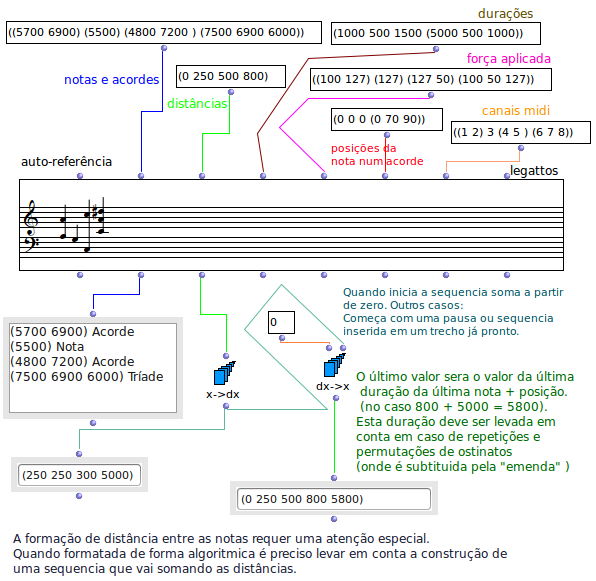
\includegraphics[scale=0.5]{OMPD/chord-seq-sem-titulo.png}
	\end{center}
	\legend{Fonte: autor }
\end{figure}



\subsubsubsection{classe permutation}

\subsubsubsection{classe math}

\subsection{PD}

OM is almost certainly now the world’s dominant
platform for doing CAC research and practice, de-
spite the presence of several other approaches (includ-
ing one, by Karlheinz Essl, that runs within Max).
Is this because OM’s design is the best, or is it that
OM has benefitted from the presence at IRCAM of
so many willing composers, such as the ones repre-
sented in this book? The two rival explanations are
impossible to extricate from one another.
\cite{puckettecomputing}

Já o Puredata, nas palavras de seu idealizador:

\begin{citacao}
Um novo sistema de software, chamado Puredata, está em seus primeiros estágios de desenvolvimento. Seu design almeja remediar algumas deficiências do programa Max e preservar algumas de suas vantagens. A mais importante fraqueza do Max é a dificuldade de manter estruturas de dados compostas de um tipo que possa ser acessado quando analisando e resintetizando sons  ou quando gravando e modificando sequencias de diferentes tipos. Também, tem sido difícil integrar sinais que não sejam de áudio (vídeo por exemplo, e também espectro sonoro ) dentro do rígido sistema de “objetos til” (~) do Max.\cite{puckette1996pure}
\end{citacao}
 

Interessante perceber que já no final dos anos 90 o PD já tinha como alvo a vindoura possibilidade de uma música performática feita com os computadores domésticos que começavam a popularizar-se, preocupando-se com aspectos de melhor performance de processamento de áudio, uso de video sincronizado e representação em tempo real de dados do de processamento sonoro, apontando para a possiblidade de outros tipos de representação da música. 

A música partiturável não era a grande preocupação e nem seus procedimentos de composição eram tão importantes quantos os aspectos relacionados ao espectro sonoro e a possibilidade de manipulação de eventos audiovisuais em tempo real.

Uma diferença prática das abordagens padrão destes sistemas: O PD não incentiva a priori o uso de algum score derivado da escala cromática, e sim parte da idéia de frequências absolutas de 0hz ao limite de sua placa de som. É orientado por controles de eventos (“bangs”) de tempo não-linear.

Além disso, os objetos tilde (~) fazem processamento de síntese sonora em tempo real, basta você plugá-los a qualquer momento em um objeto que representa sua placa de som processando vetores numéricos indicando a pressão e descompressão do seu auto-falante em estado bruto, o [dac~]. No OM é sempre necessário compilar (“verificar”) os patches para depois ouvi-los em sequenciadores de eventos ou players de áudio.

Miller Puckette comenta num artigo de 2006 que o uso de procedimentos 

I would like to see some of the techniques now only available in OM become usable some day within
real-time environments. This is clearly a huge undertaking, since the style of programming currently used
in real-time applications is so different from that in OM. But there would be much gained if this became
possible. In the meantime it’s possible to send messages back and forth between OM and some lower latency process that takes care of real-time performance. 
\cite{puckettecomputing}



\subsubsection{biblioteca Maxlib}

\subsubsection{biblioteca RTC-lib}

\subsubsection{objeto [probalizer]}



% ----------------------------------------------------------
\chapter{Arquivos e Scripts para Segmentação de Dados Musicais}
% ----------------------------------------------------------
\label{formatos}

\section{MIDI}

Por muito tempo o formato MIDI ficou estigmatizado por ser associado aos timbres genéricos da indústria de sintetizadores populares dos anos 80 e 90 e pelas primeiras placas de som e softwares sequenciadores de eventos ou partituras dos computadores pessoais. 
Na verdade o formato não carrega parâmetros de timbres em seus metadados. Arquivo MIDI valores básicos de expressão e alturas cromáticas do gestual de uma performance instrumental, permitindo que esta seja posteriormente associada a qualquer timbre.

A mensagem MIDI básica carrega informação sobre:

\begin{enumerate}

\item O canal onde vai atuar permitindo mixar diversos instrumentos em polifonia.

\item O programa que indica o timbre.

\item NoteOn/NoteOff - Nota soando , nota sem soar. o MIDI manda duas informações básicas sobre o envelope da nota. Uma primeira nota com a força inicial e o uma segunda com a mesma nota e força zero, para silenciá-la.

\item "Velocity" ou expressão: força com qual a nota é tocada.

\item Canal de controle para uso de escala de 127 passos que tem uso dependente da implementação da aplicação. Por exemplo, parâmetros de equalização timbre. Na prática o canal de controle é geralmente usado para receber dados de potenciômetros ou sensores analógicos e assinalado a qualquer tipo de parâmetro.

\item Pitch Bend - Parâmetro para atuar diretamente na afinação de uma nota em tempo real, de modo similar ao gesto de bend de instrumentos de cordas. A especificação midi permie que este controle tenha uma granulação de 16.384 pontos e geralmente é usada para um slide que cobre duas oitavas.

\item Mensagens exclusivas de sistema (SysEx) geralmente usadas por aplicações para ações independentes do gesto musical, por exemplo informar ao sistema onde onde buscar arquivos temporários de uma sessão.
\end{enumerate}

É importante ter em mente que os arquivos MIDI, por ser há mais 35 é um padrão ainda em uso, gerou um legado relevante de arquivos baseados em repertório clássico para a reconstituição de corpus de peças partituradas. Porém não são descritores capazes de garantir a boa formatação de seus dados como figuras de compasso de uma pauta tradicional, já que os arquivos MIDI não carregam informações sobre as figuras, apenas sobre suas durações, alturas e expressão. Quando importados para programas de notação ou convertidos para formatos destes, os arquivos MIDI irão passar por uma segmentação arbitrária e determinada pelo algoritmo "parser"\footnote{definir parser} que vai converter determinada duração em determinada métrica quantizada, normalmente diferente das articulações de quais as músicas foram digitalizadas.


Veremos a seguir outros arquivos mais específicos para este fim e quando necessário será feita a conversão entre os tipos.



\pagebreak

\section{Lilypond}

O objetivo principal aqui é a formatação de uma notação partitural avançada e otimizada para impressão em papel. Permite também a utilização de elementos de notação mais exótica, inclusão de texto, dedilhados, nomenclatura de acordes, sinais de expressão, e customização de elementos a partir de módulos. Facilita a otmização da disposição e dimensão das fontes dos objetos e possui uma linguagem script própria dialeto da sintaxe scheme\footnote{Tutorial oficial de lilypond-scheme: \url{http://lilypond.org/doc/v2.16/Documentation/source/Documentation/extending/introduction-to-scheme}}.



\begin{figure}[htb]
	\caption{\label{fig_grafico}Gerador de um acorde Dó maior (dó4 e4 g5) na clave de sol em Lilypond}
	\begin{center}
	    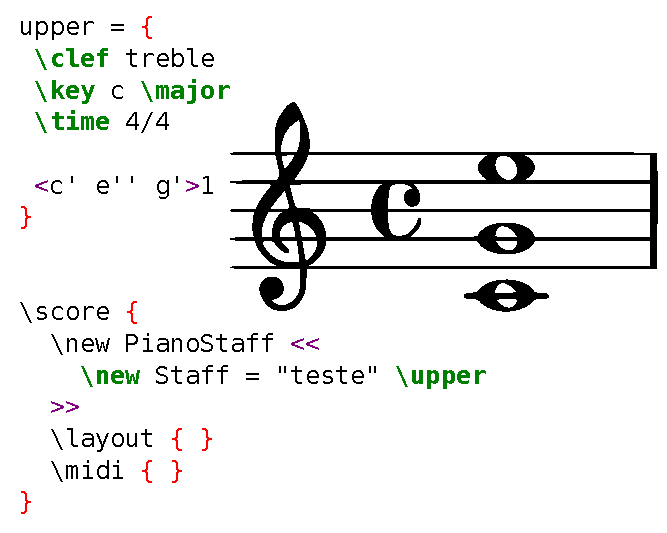
\includegraphics[scale=0.75]{score/lilypond.pdf}
	\end{center}
	%\legend{Fonte: autor}
\end{figure}




\section{MusicXML}

O uso geral do formato MusicXML é similar ao Lilypond - formatação de partituras. No entanto, enquanto Lilypond é um sistema completo fechado em si próprio, o MusicXML é um formato com a intenção de tornar-se um padrão intercambiável entre diferentes aplicações de partitura\footnote{ Lista atualizada de aplicações compatíveis com o formato MusicXML: \url{http://www.musicxml.com/software/} }.


\begin{figure}[htb]
	\caption{\label{fig_grafico}Gerador de uma nota dó4 na clave de sol em MusicXML}
	\begin{center}
	    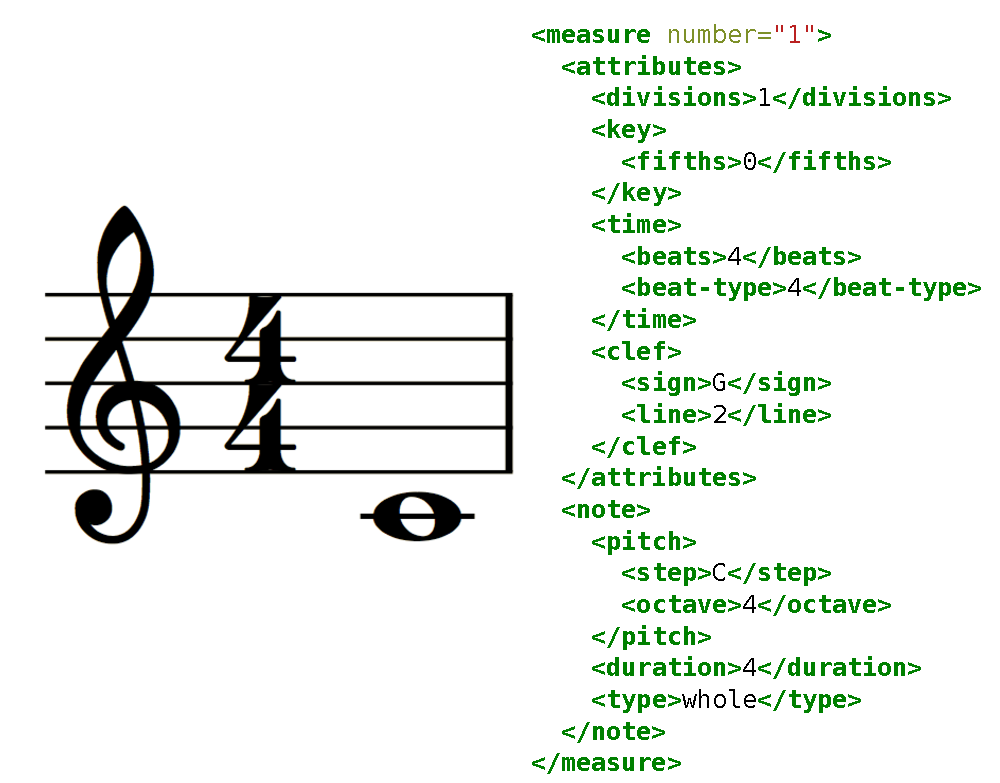
\includegraphics[scale=0.5]{score/musicxml.pdf}
	\end{center}
	%\legend{Fonte: autor}
\end{figure}

\pagebreak
\section{Bibliotecas Python auxiliares}

Pela sua natureza de código aberto alto-nível de orientação a objetos, Python\cite{van1995python} é uma linguagem script que tem sido amplamente adotada e ampliada por bibliotecas para as mais diversas aplicações científicas.\cite{downey2009python}

Aliada ao uso de algumas bibliotecas específicas para arquivos de segmentação partitural, Python mostra-se uma ferramenta prática para formatação dinâmica de partituras prontas para impressão ou para auxiliar a análise de dados quantitativos de corpus de partituras.

Falaremos a seguir de duas dessas bibliotecas utilizadas como ferramenta auxiliar nesta pesquisa:


\subsection{Abjad}

É uma biblioteca voltada para a formatação de clichês em notação partitural pronta para impressão em papel, baseada na manipulação de templates no formato lilypond. A biblioteca apresenta alguns templates baseados em peças de Bártok, Ligeti, Ferneyhough e Mozart.



\subsection{Music 21}









% ----------------------------------------------------------
% PARTE
% ----------------------------------------------------------
\part{Paradigmas para uma Análise Musical Pós-Tonal}
\label{analises}
% ----------------------------------------------------------




% ---
% Capitulo de revisão de literatura
% ---
\chapter{Formalização linguística de gramáticas musicais }

Em seu ensaio "A comparação das análises sobre o ponto de vista semiológico", J.J. \citeonline{nattiezcomparaccao} faz um balanço das diferentes abordagens analíticas na musicologia 

\begin{citacao}
As diversas práticas da análise musical no século XX podem, na minha opinião, estar, de início, repartidas em duas grandes categorias, (...): 

1. Aquelas que admitem – e mesmo sublinham – as conotações emotivas, afetivas, imagéticas da obra musical. Designarei as mesmas com o termo genérico e moderno de análises de orientação semântica. (...)\linebreak
2. Aquelas que se apoiam sobre as estruturas imanentes da obra e que se repartem em dois grandes grupos: a. \textbf{as análises taxionômicas que cortam em unidades a substância musical, privilegiando este ou aquele parâmetro. }(...) b. \textbf{As análises que, na falta de melhor termo, chamarei “lineares” e que, (...), 
descrevem o prolongamento e as implicações das alturas, tanto no nível melódico (...), quanto no harmônico (...)}
\cite[grifos nossos]{nattiezcomparaccao}
\end{citacao}


% ---
Buscaremos aqui alguns caminhos para entender que procedimentos podem ser essenciais para a formalização de gramáticas musicais computáveis. Nossa intenção principal é encontrar um fio condutor para a didática de algoritmos composicionais e analíticos para a música que deem conta de estruturas da música pós-tonal anterior aos experimentos com timbre e música concreta que foram determinantes na segunda metade do século XX.  

Partiremos de uma pequena revisão histórica e conceitual da aplicação do termo "gramática" no contexto da computação musical e suas derivações e implicações.  

Utilizaremos o termo “gramática” em sentido mais estrito e para isso tomamos como ponto de partida o entendimento deste termo dentro das ciências computacionais. Em paralelo iremos pensando como este modelo influenciou a formalização de gramáticas musicais estruturalistas e quais alternativas vão aparecendo como adjacentes para formalização de algoritmos musicais.

O modelo de racionalização da linguística iniciado por Noam Chomsky com a obra "Syntactic Structures" \cite{chomsky1957syntactic} e formalizado na sua "Teoria da Sintaxe"\cite{chomsky1965aspects}  até hoje é uma das bases para o estudo algorítmico e algébrico de processamento linguagens naturais.  

Sua influência na teoria musical pode ser encontrada em muitas tentativas de aproximar linguística e musicologia nas década de 70 e 80.

Inspirou as formalizações rígidas de modelos da musicologia da cognição inspirados na linguística na “Teoria Gerativa da Música Tonal” \cite{lerdahl1983generative} - um trabalho interdisciplinar do linguista Ray Jackendoff com o musicólogo Fred Lerdahl que detalharemos mais adiante.

Uma abordagem curiosa para comparação desta mesma época é a de Leonard Berstein na série de palestras “Unswared Question” \cite{bernstein1976unanswered}. Sua especulação empírica foi bastante alegórica e demonstrada inventivamente ao piano em seu registro em vídeo. Bersnstein fez comparações das estruturas de ordenamento das frases escritas e faladas com montagens de sessões motívicas de peças clássicas e chega a fazer algumas metáforas entre classes gramaticais e funções de acordes. Este tipo de metáfora parece ser de fato uma das motivações iniciais da pesquisa neste campo, porém muita coisa foi problematizada de maneira mais rigorosa, buscando métodos quantitativos, e nos anos seguintes contribuiu para as bases de organização de uma disciplina hoje conhecida por "cognição musical".

Pelo bem ou pelo mal, a abordagem de Bernstein parece estar muito mais para o universo das analogias poéticas livres do que a busca por uma formalização strictu sensu \cite{lerdahl2009genesis} como a que se sucedeu nas derivações das gramáticas gerativas musicais \cite{lerdahl1983generative,temperley2004cognition} ou em formulações algébricas e algoritmicas que Curtis \citeonline{roads1979grammars} já apontava em seus estudos da época.

 

\section{Gramáticas Musicais Computáveis}

Uma interessante e histórica análise no ensaio de Curtis \citeonline{roads1979grammars} é um panorama que fez sobre o estado da arte da influência da linguística sobre musicologia na época, fazendo um estudo comparado dos trabalhos de \citeonline{smoliar1976music,lindblom1970towards,laske1977music, winograd1968linguistics, moorer1972music, nattiez1977fondements,ruwet1975theorie, lerdahl1983generative} e o próprio trabalho anterior de \citeonline{roads1978composing}.


O interessante deste panorama é que coloca lado a lado perspectivas mais empíricas como de \citeonline{nattiez1977fondements} e \citeonline{ruwet1975theorie} e outras que buscavam efetivamente uma inspiração para um rigor computacional de sintaxes musicais. Vale lembrar que Nattiez também tem um estudo comparado da influência da linguística na musicologia, com um ponto de vista menos pragmático e mais historicista, muito mais abrangente, e que traz um ponto de vista bem mais recente \cite{nattiez2004modelos} do que decorreu a seguir.


Segundo Roads, \citeonline{moorer1972music} e \citeonline{winograd1968linguistics} chegam a realizar alguns experimentos computacionais. \citeonline{smoliar1976music} toca num ponto tecnologicamente complexo para a época: a segmentação de arquivos sonoros diretamente a partir de gravações. 

\citeonline{laske1977music} propõe analogias com a fonologia (relação entre sintaxe e sons da palavra falada) com uma recente “sonologia” (relação de uma sintaxe musical e os sons musicais). A dupla\citeonline{lerdahl1983generative}  investe numa normatização bastante inspirada nas segmentações propostas por Chomsky e procura problematizar aspectos de uma cognição musical tonal, que teria bases culturais sólidas na tradição ocidental, que veremos a seguir na \autoref{GTTM}.



\chapter{Teorias Cognitivistas para uma Segmentação Tonal}

\section{Gramática Gerativa da Música Tonal (GTTM)}
\label{GTTM}

Jean Jaques Nattiez, em seu ensaio sobre música e linguística \cite{nattiez2004modelos} relativiza também o êxito do texto de Lerdahl e Jackendoff, porém reconhece uma importância  que despertou nossa curiosidade por uma pequena revisão nas regras propostas por esta obra, o que faremos logo a seguir.

\begin{citacao}
Porque, se a obra de Lerdahl e Jackendoff não conheceu um amplo reconhecimento sob o ponto de vista da análise das obras stricto sensu, em compensação, a psicologia cognitiva da música, que sabemos estar em plena efervescência, (…) Na medida em que 51 das 56 regras propostas são dadas como universais \cite[ p.345-352]{lerdahl1983generative}, os autores lançam aos etnomusicólogos um grande e salutar desafio que ainda não foi levado em consideração. A importância de um trabalho não se mede unicamente por seu caráter inovador e pelo valor dos modelos propostos, o que, por certo, ocorre neste caso, mas também pelo campo de investigações novas que propõe.
\cite{nattiez2004modelos}
\end{citacao}


O que buscamos como objeto no presente trabalho é um percurso composicional utilizando algum repertório significativo de critérios analíticos com enfase em abordagens que busquem métodos para extrair regras gerativas
\footnote{
Lerdahl e Jackendoff colocam o termo “gerativo” ( que é derivado da linguística ) de uma forma que não signifique a príncipio uma fórmula capaz de gerar aquela música, mas sim um estrutura pela qual a escuta já experimentada naquela cultura musical guia-se para segmentar e fruir sua sixtaxe. \cite[ p.6]{lerdahl1983generative}
}
que estejam estruturalmente passíveis de serem descritas em forma de algoritmos. 

Para isso iniciamos refletindo sobre uma das mais influentes teorias musicais com parentesco na linguística estruturalista e as tentativas de encontrar fórmulas de sintaxe para compreender os mecanismos seletivos da cognição musical: “A Teoria Gerativa da Musica Tonal”, conhecida por “GTTM”, sigla do termo inglês “Generative Theory of Tonal Music” \cite{lerdahl1983generative}.

A GTTM introduz uma taxonomia para separar de um plano musical seus agrupamentos melódicos, harmônicos e ritmicos, buscando uma maneira estruturada para fazer uma segmentação hierárquica de motivos que supostamente estariam dentro de uma previsibilidade de uma escuta ocidental tonal, apontando limitações e contradições entre estas regras e buscando apoiar-se em processos cognitivos rastreados pela audição, psicoacústica e cultura desta escuta. 

Desta maneira também problematiza e limita para fora do seu escopo peças que podem esconder segmentações registradas em esquemas composicionais anteriores a realização das obras, com estruturas racionalizadas porém fora do plano auditivo e cognitivo mais básico e intuitivo na cultura tonal ocidentalizada. 

\pagebreak
%%%%%%%%%%%%%%%%%% gttm esquema
\begin{figure}[!h]
	\caption{\label{fig_grafico}Fluxograma de \citeonline{lerdahl2009genesis} para a GTTM}
	\begin{center}
	    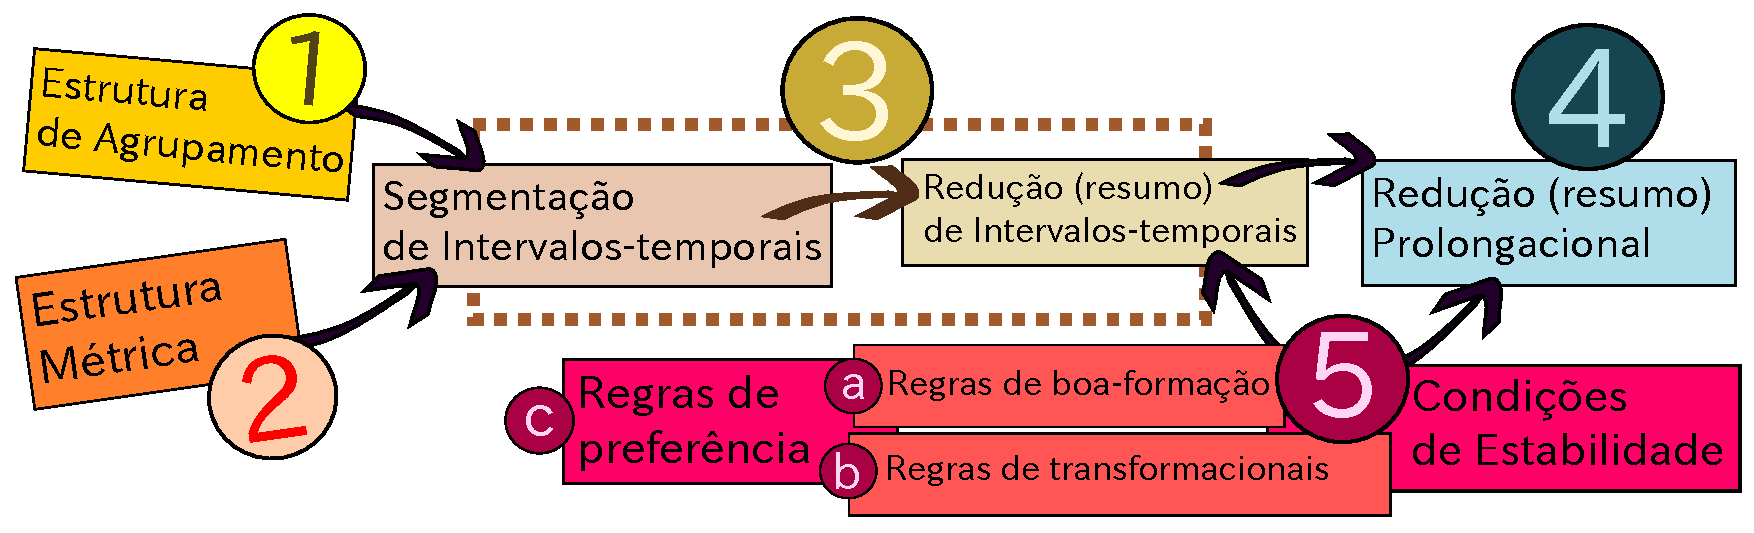
\includegraphics[scale=0.5]{gttm/GTTM_rules.pdf}
	\end{center}
	\legend{Fonte: \citeonline[p. 2 , tradução do autor]{lerdahl2009genesis}}
\end{figure}


\begin{citacao}
A teoria [GTTM] clama que, se um sinal permite, o ouvinte inconscientemente infere quatro tipos de estruturas hierárquicas de uma superfície musical:\linebreak 
\textbf{1.} estrutura de agrupamento, ou a segmentação do fluxo musical em unidades como motivos, frases e sessões; 
\textbf{2.} estrutura métrica, ou padrão de batidas recorrentes periodicamente forte e fracas associadas com a superfície; 
\textbf{3.} redução de intervalo temporal, ou a importância estrutural relativa dos eventos como são ouvidos dentro do contexto estabelecido pelas unidades rítmicas; e
\textbf{4.} redução prolongacional, ou os padrões percebidos pela tensão e relaxamento ao longo dos eventos em vários níveis da estrutura \cite{lerdahl1992cognitive}
\footnote{
"The theory claims that, if the signal permits, the listener unconsciously infers four types of hierarchical structure from a musical surface: grouping structure, or the segmentation of the musical flow into units such as motives, phrases, and sections; metrical structure, or the pattern of periodically recurring strong and weak beats associated with the surface; time-span reduction, or the relative structural importance of events as heard within contextually established rhythmic units; and prolongational reduction, or the perceived pattern of tension and relaxation among events at various levels of structure"\cite{lerdahl1992cognitive}

}
\end{citacao}

\subsection{Regras de boa formatividade dos agrupamentos (GWFRs)}

%%%%%%%%%%%%%%%%%% mozart
\begin{figure}[htb]
	\caption{\label{fig_grafico}Agrupamento de motivos do início da sinfonia K550 de Mozart.}
	\begin{center}
	    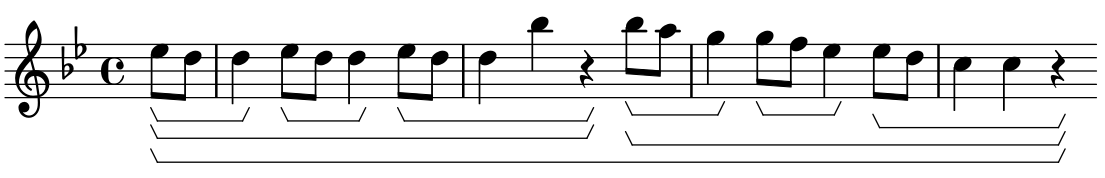
\includegraphics[scale=0.45]{gttm/lilypondGROUPmozartGTTM.png}
	\end{center}
	\legend{Fonte: \cite{lerdahl1983generative} }
\end{figure}

\begin{citacao}
GWFR 1 “Qualquer sequencia contígua de eventos de alturas, batidas percussivas, ou similares constituem um grupo, e somente sequencias contíguas constituem um grupo” \cite[ pg.37]{lerdahl1983generative}.
\end{citacao}

Esta regra estabelece que este tipo de escuta irá selecionar agrupamentos apenas por eventos sequenciados, não valendo por exemplo agrupar sons por estarem na mesma oitava ou por serem de figuras rítmicas iguais, pois isto implicaria em uma seleção cognitiva-auditiva de eventos num tempo não-linear, desconstruindo a escuta proposta pela sequencia de eventos da composição original.

As próximas regras de boa formatividade concluem por conjunção que os grupos se estabelecem por uma hierarquia de pequenos grupos contidos em grupos maiores, onde sempre um grupo grande pode ser decomposto em grupos menores:


\begin{citacao}
GWFR 2 “Uma peça contem um grupo”\linebreak
GWFR 3 “Um grupo deve conter grupos menores”\linebreak
GWFR 4  “Se um grupo G1 contém G2 ele deve conter G2 inteira” 
 \cite[ p.38]{lerdahl1983generative}
\end{citacao}


%%%%%%%%%%%%%%%%%% mal formados
\begin{figure}[htb]
	\caption{\label{fig_grafico}Exemplos de agrupamentos “mal formados” de acordo com a regra GWFR5}
	\begin{center}
	    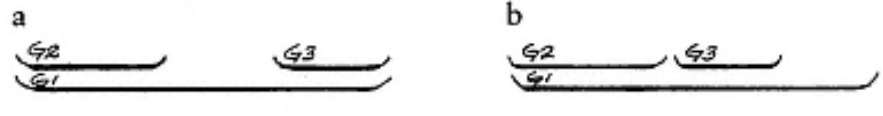
\includegraphics[scale=0.35]{gttm/GWFR_fig33.png}
	\end{center}
	\legend{Fonte: \cite{lerdahl1983generative} }
\end{figure}




\begin{citacao}
GWFR 5 “Se o grupo G1 contém grupos menores , então ele deve ser exaustivamente particionado em pequenos grupos”
\cite[ p.38]{lerdahl1983generative}
\end{citacao}

\subsubsection{Regras de preferência para agrupamentos (GPRs)}

\begin{citacao}
GPR1 “Evite analises com pequenos grupos, quanto menor menos preferível”.
\cite[ p.43]{lerdahl1983generative}
\end{citacao}


Segundo a GTTM pequenos grupos geralmente não serão capazes de sozinhos estabelecer contextos. Uma pequena digressão: Isto seria questionável em uma teoria que considerasse pequenos motivos como uma espécie de "objeto sonoro"\footnote{c.f. \cite{guigue1995analise}} , mas não é o caso desta abordagem, que está preocupada com uma camada exterior que supostamente é edificada por esta articulação contígua de grupos internos. A ideia de um pequeno motivo que irrompe esta superfície funcional linear como uma sonoridade\footnote{c.f. \cite{guigue2012}} articulada como entidade é extremamente interessante, mas por hora ficará fora do escopo.

\begin{citacao}
GPR2 “(Proximidade) – Considere uma sequencia de quatro notas [n1-n2-n3-n4].\linebreak
O restante sendo igual, a transição n2-n3 deve ser considerada uma fronteira de segmento se:\linebreak
a) (Ligadura/Pausa) o intervalo-temporal desde o final de n2 ao ínicio de n3 é menor do que desde final de n3 ao início de n4.\linebreak
b) (Ponto-de-ataque) o intervalo-temporal entre os pontos de ataque entre n2-n3 é maior do que entre n1-n2  e entre n3-n4.
\cite[ p.45]{lerdahl1983generative}
\end{citacao}

Esta regra é centrada na busca por rupturas no fluxo dos motivos, isolando as frases pelos pontos de ataque fortes, ligaduras ou intervalos claros entre dois motivos.  


É notória a semelhança desta regra com o procedimento que aprendemos desde a alfabetização gramatical para a “separação de sílabas” - a procura de “respiros” das frases. 


A busca de critérios para uma segmentação intuitiva destes “respiros” entre os motivos vai permear de alguma forma todo esforço da GTTM. 

\begin{citacao}
“Mas, precisamente, o que a comparação atenta da linguagem verbal e da música nos ensinou, é que a significação em música não tem o mesmo estatuto que na linguagem.”\cite[ p.9]{nattiez2004modelos}
\end{citacao}

Quanto a analogia com os critérios de segmentaçao da língua escrita e falada, percebemos na GTTM e outros trabalhos Lerdahl(1992, 2003, 2013) um descrédito quanto ao fato que a música poderia simplesmente transpor metaforicamente as regras transformacionais da linguistica chomskiana, como por exemplo nas separações por classes gramaticais em complementos nominais e complementos verbais.  De fato para tal percurso seria necessário uma certa “licença poética” mais abitrária.1

Por outro lado, mesmo com todo rigor metodológico, seria preciso pensar todas características para além do aparecimento temporal dos eventos

Além do “respiro” passamos a levar em consideração alguns critérios de modificação do som como altura, força do ataque, gestual da articulação e o envelope de duração nas emendas dos segmentos.

\begin{citacao}
GPR3 (Mudança) Considere uma sequencia de notas [n1-n2], a transição [n2-n3] deve ser ouvida como um grupo de fronteira se marcado por:
a) registro – a transição n2-n3 envolve uma maior distância intervalar de que entre n1-n2 ou n3-n4,\linebreak
b) dinâmica - a transição n2-n3 envolve uma mudança dinâmica maior de que entre n1-n2 ou n3-n4,\linebreak
c) articulação - a transição n2-n3 envolve uma mudança de articulação maior de que entre n1-n2 ou n3-n4,\linebreak
d) duração - há diferença de durações  entr n2-n3 enquanto n1-n2 ou n3-n4 permanecem com durações similares,
\cite{lerdahl1983generative}
\end{citacao}

\begin{figure}[htb]
	\caption{\label{fig_grafico}Open Music 01}
	\begin{center}
	    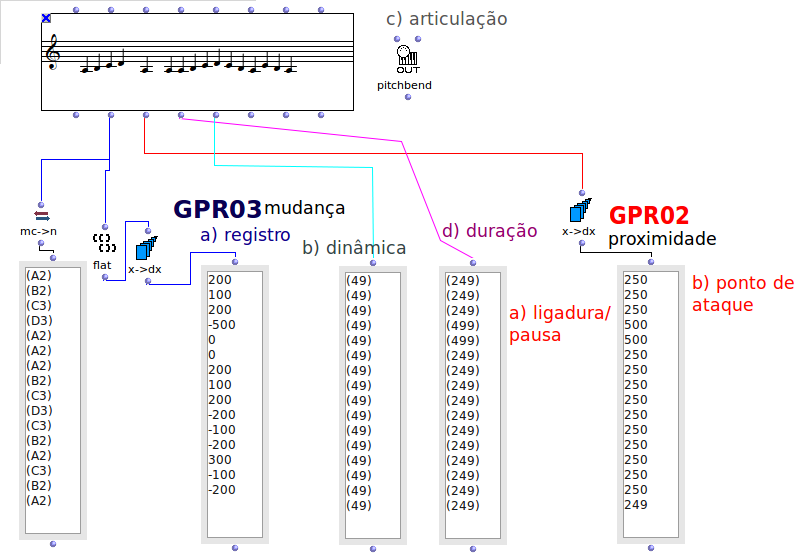
\includegraphics[scale=0.5]{mikro/OM_gttm_GPR02-03.png}
	\end{center}
	\legend{Fonte: autor }
\end{figure}






As regras seguintes especializam as GPRs anteriores, filtrando agrupamentos que tendem a ficar em níveis mais frasais do que os pequenos motivos que deverão conter em sua composição:

\begin{citacao}
GPR4 (Intesificação) Onde os efeitos dos GPR 2 e 3 são relativamente mais pronunciados, um grupo de nível mais largo deve ser localizado.\linebreak
GPR5 (Simetria) Prefira análise de agrupamentos com a abordagem mais próxima da subdivisão de grupos em partes de duração iguais.\linebreak
GPR6 (Paralelismo) Onde dois ou mais segmentos musicais podem ser construídos em paralelo, eles preferivelmente formam partes paralelas dos grupos\linebreak
GPR7 (Estabilidade de prolongacional e de intervalo-tempo ) Prefira uma estrutura de agrupamento em um intervalo-tempo tempo mais estável e/ou reduções prolongacionais
\cite[ pg.46-52]{lerdahl1983generative}
\end{citacao}

As regras a seguir problematizam um ponto que é interessante a comparação entre as gramáticas musicais e as verbais. Em música é inevitavel que em certos momentos uma nota ou acorde ou tempo forte de pausa de um motivo “emende no próximo” (Sobreposição), o que poderia acontecer sonoramente em linguagem coloquial apressada, mas nunca na língua escrita, como por exemplo aglutinar uma estrutura substantivo-adjetivo criando uma palavra emendada por fonemas finais e iniciais como “cobrAzul” ou “barulhOrrível”. Uma variação possível de analogia seria com uma emenda de uma frase inacabada onde a nova palavra parece chegar “adiantada”, semelhante ao que acontece no substantivo composto “copo d'água”. 

%%%%%%%%%%%%%%%%%% gttm elisao
\begin{figure}[htb]
	\caption{\label{fig_grafico}Elisao ou Contração}
	\begin{center}
	    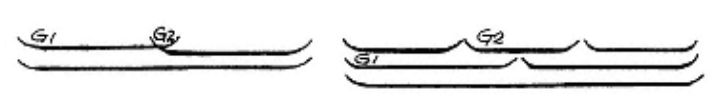
\includegraphics[scale=0.5]{gttm/GWFRfig32.png}
	\end{center}
	\legend{Fonte: \citeonline[p. 2]{lerdahl1983generative}}
\end{figure}

%%%%%%%%%%%%%%%%%% elisao overlay gestalt
\begin{figure}[htb]
	\caption{\label{fig_grafico}Formalização visual dos problemas de elisão e sobreposição de camadas na GTTM. \cite[ p.69]{lerdahl1983generative}}
	\begin{center}
	    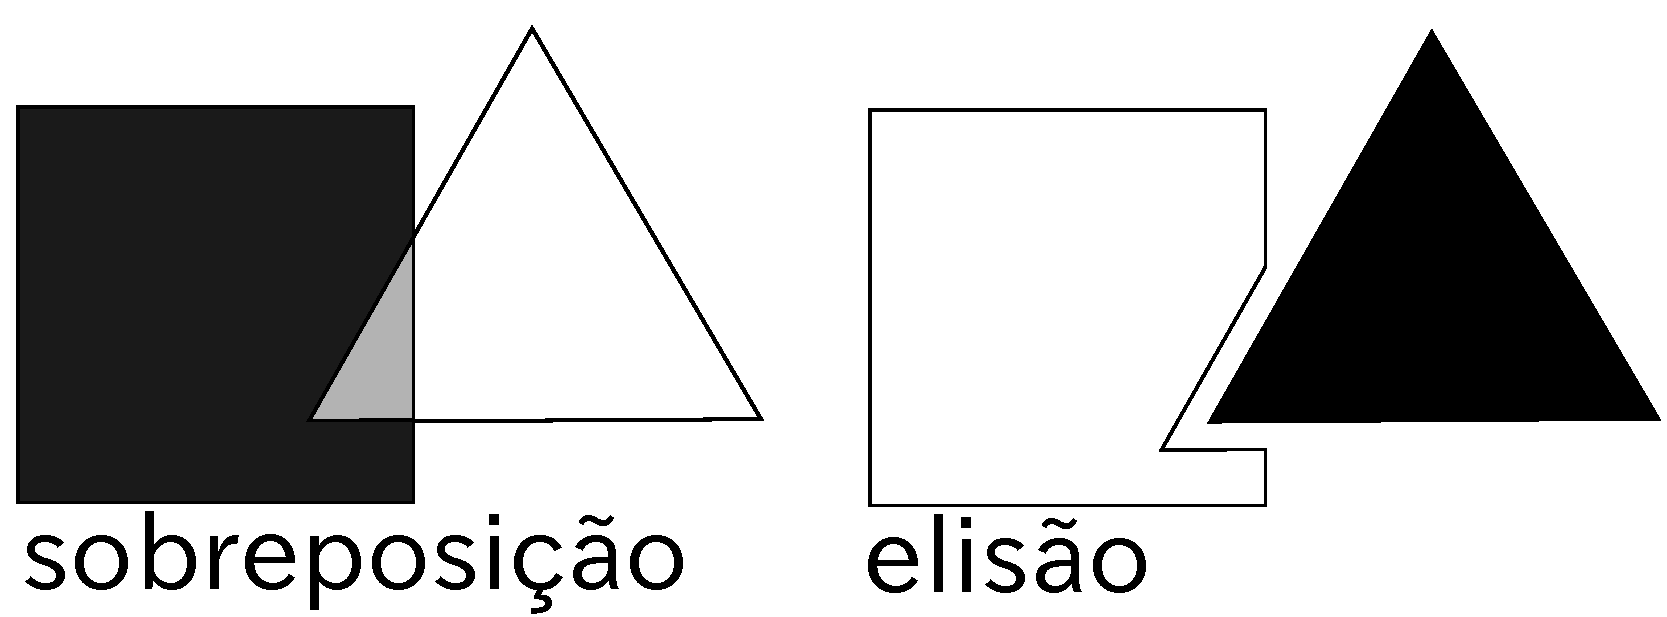
\includegraphics[scale=0.25]{gestalt/gestalt_elision_overlay.pdf}
	\end{center}
	\legend{Fonte: autor}
\end{figure}



“Estes exemplos visuais parecem não ser apenas analogias triviais ao fenômeno musical. Como nas discussões de regras de preferência, a possibilidade de traçar paralelos entre os domínios auditivo e visual apontam a operação de processos fundamentais de da percepção e/ou cognição.” \cite{lerdahl1983generative} 3

\subsection{Regras de boa-formação métrica (MWFRs )}

Antes de entrar na taxonomia das regras de boa formação métrica convém entender o que a GTTM coloca como “acento”. Há uma categorização que divide os acentos em fenomenológico , estrutural, ou métrico.4 

Por fenomenológico os autores entendem acentos que são causados por eventos marcantes e destacados da superfície musical como pontos extremos no contorno melódico, stress ou relaxamento súbito nas articulações ou pontos de tensão inesperada na harmonia, estruturais seriam acentos bem marcados pelas cadências de progressões harmônicas mais marcantes e esperadas.

Métricos seriam os acentos que intuitivamente estariam no pulso intuitivo da superfície musical, nos tempos fortes e síncopas e que de alguma maneira reforçam uma marcação rítmica esperada pela peridiocidade dos eventos. 

Os autores não associam diretamente este tipo de acento a uma declaração de assinatura de compasso na escritura da peça, mas sugerem que de alguma maneira este tipo de acento é justamente uma relação de afirmação ou negação dessa possibilidade de haver uma peridiocidade forte nos eventos, que a escritura tentaria prever. 


%%%%%%%%%%%%%%%%%% ritmica gttm
\begin{figure}[htb]
	\caption{\label{fig_grafico}Notação analítica proposta pela GTTM que marca uma hierarquia das batidas por subdivisões de pulsos}
	\begin{center}
	    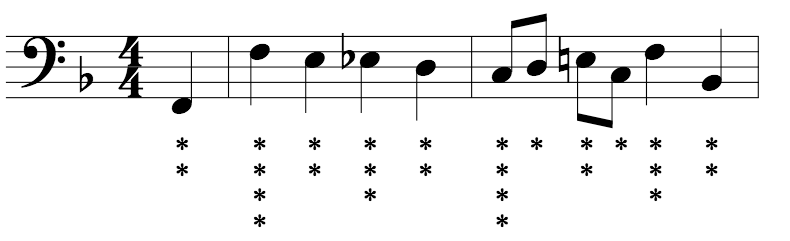
\includegraphics[scale=0.45]{gttm/GTTM-m21-metes.png}
	\end{center}
	\legend{Fonte: autor}
\end{figure}


As regras de boa formação métrica na GTTM estabelecem as condições mínimas para que o efeito de periodicidade aconteça.  Observa-se que se por uma lado a escrita tradicional com seus compassos e assinaturas serve como um ponto de partida e apoio para contagem de batidas baseadas nas subdivisões das figuras métricas ela também é fator limitador na redução dos intervalos-temporais. Este problema aparece na GTTM como “apagamento métrico”(idem, pg.101), algo similar a colisões e elisões vistas nos agrupamentos. 

Não é por acaso que a partir do século XX a escrita com mudanças constantes de assinatura de compasso chega em um ponto, após o serialismo integral principalmente, em que propõe-se a abolição da assinatura ou barra de compassos num extremo e no outro extremo uma complexidade tão alta na subdivisão de quiálteras que ficam totalmente arbitrários e subentendida na notação uma indução ao improviso do interprete.

Voltando às regras, como no agrupamento, na métrica também temos as regras de boa formação (WFRs - “Well Formed Rules”) para os casos mais gerais e em seguida atemos as regras de preferência (PRs - “Preference rules”) hierarquizando as decisões.

\begin{citacao}
MWFR 1 "Todo ponto de ataque deve estar associado a uma batida de nível métrico menor presente naquele ponto da peça" 
MWFR 2 "Toda batida em dado nível deve também ser uma batida em níveis menores daquele presente ponto da peça" 
MWFR 3 "A cada nível métrico, batidas fortes são espaçados por uma separação de duas ou três batidas" 
MWFR 4 "O tátil e o material imediatamente mais largo devem consistir de batidas igualmente espaçadas através da peça. No nível subtátil, batidas fracas devem estar igualmente espaçadas entre as batidas fortes que os cercam." 
 \cite{lerdahl1983generative}
\end{citacao} 

\subsubsection{Regras de preferência Métrica (MPFRs) } 

\begin{citacao}
MPFR1 (Paralelismo) "Onde dois ou mais grupos ou partes de grupos podem ser construídos em paralelo, eles preferivelmente recebem uma estrutura métrica paralela" 
MPFR2 (Batida forte adiantada) "Prefira raramente uma estrutura métrica onde a batida mais forte em um grupo aparece relativamente adiantada no grupo" 
MPFR3 (Evento) "Prefira uma estrutura material onde as batidas do nível Li coincidem com a inserção de eventos de altura nas batidas fortes de Li" 
MPFR4 (Tensão) "Prefira uma estrutura métrica onde as batidas do nível Li são tensionadas com as batidas fortes de Li" 
MPFR5 (Duração) "Prefira uma estrutura métrica onde batidas relativamente fortes ocorrem na inserção de também relativamente longos: 
a) evento de altura 
b) duração de dinâmica 
c) ligadura 
d) padrão de articulação 
e) duração de um pitch em níveis relevantes da redução intervalo-temporal 
f) duração da harmonia em níveis relevantes  da reduação intervalo-temporal (ritmo harmônico )

MPFR6 (Baixo) "Prefira um baixo metricamente estável" 
MPFR7 (Cadência) "Prefira fortemente uma estrutura métrica onde as cadências são metricamente estáveis; ou seja, evite fortemente violações das regras de preferência locais que possuem cadências" 
MPFR8 (Suspensão) "Prefira fortemente uma estrutura métrica onde a suspensão é uma batida mais forte que a resolução" 
MPFR9 (Interação intervalo-temporal) "Prefira uma análise metrica que minimize o conflito na redução do intervalo-temporal" 
MPFR10 (Regulação Binária) "Prefira estruturas métricas em que em cada nível toda a outra batida seja forte" 
 \cite{lerdahl1983generative}
\end{citacao}



\section{Segmentação temporal de eventos cadenciais e a redução prolongacional na GTTM}


É importante destacar a partir daqui que as continuidades e derivações da pesquisa iniciada pelo GTTM tiveram que buscar fórmulas mais rigorosas em pesquisas quantitativas sobre "cognição das alturas musicais"\cite{krumhansl1990cognitive} nos níveis de interação entre as camadas melódico-harmônica com os agrupamentos métrico-rítmicos para sustentar seus argumentos sobre as preferências condicionadas do tal "ouvinte experiente"\cite[pg. 118]{lerdahl1983generative} como fator organizador da teoria. 

As regras de redução prolongacional, similares aos resumos cadenciais shenkerianos que segmentam os eventos melódico-harmônicos, são dependentes daquilo que a GTTM chama de intervalo-temporal ("time span") - regras de preferência determinadas por fatores internos da superfície musical: proximidade de uma tônica, modulação de regiões funcionais de tonalidade, âmbito de registro de oitava, paralelismo motívico e toda uma suposta hierarquia destas interações. No entanto estes apontamentos foram desde então criticados por sua arbitrariedade indutiva.\footnote{ c.f. "Pontos típicos da crítica " da GTTM em \cite[pg. 35]{hansen2011legacy} }

O próprio \citeonline{lerdahl2009genesis} afirma em sua revisão da GTTM:

\begin{citacao}
The interaction principle itself may still be too techni-
cal to be tested empirically at this point; but its larger
context, the perception of hierarchical pitch structures,
is a topic of considerable interest to music psychology.
GTTM’s prolongational component, however, presents
difficulties in this regard. (...)
The solution began to take shape with the development
of pitch-space theory \cite{lerdahl1988tps}, which
quantifies the most important of the stability condi-
tions through computational modeling of empirical
data on the tonal hierarchy (Krumhansl, 1983, 1990).
The idea is that the cognitive distance of an event from
a given reference point measures the instability of that
event in relation to the reference point. On the assump-
tion that the listener unconsciously seeks the most sta-
ble construal of a musical passage, TPS’s principle of
the shortest path selects events yielding the smallest
available distances from superordinate events at each
stage of prolongational reduction.
\cite[p. 191]{lerdahl2009genesis}
\end{citacao}

Decidimos portanto não entrar em detalhes destes dois escopos mais frágeis da GTTM e focaremos diretamente em derivações posteriores que os problematizam em outros termos. Tomaremos dos estudos de Lerdahl posteriores ao GTTM  por enquanto apenas seu conceito de tensão e estabilidade desenvolvido em sua "teoria do espaço tonal"("Tonal Pitch Space", doravante referida como TPS) na próxima sessão. Em seguida apresentamos uma alternativa derivada da GTTM, elaborada por David Temperley e implmentada computacionalmente em seu trabalho "Cognition of Basic Musical Structures"\cite{temperley2004cognition}.




\subsubsection{Calculando a tensão e o Espaço das alturas tonais (TPS) }



\begin{citacao}
The tonal hierarchy- hence an implicit pitch space- appears in GTTM
in incomplete form under the rubric of verbally stated stability conditions.
The theory claims that listeners cannot infer complex event hierarchies
without having access to such conditions, which are the main source for
ranking the relative stability of events within embedded temporal regions.
These regions in turn derive directly or indirectly from the grouping and
metrical structures. Figure 1 illustrates schematically that the time-span re-
duction derives from the rhythmic components and the stability conditions,
and the prolongational reduction derives from the time-span reduction and
the stability conditions. In short, both a rhythmic framework and criteria
for pitch stability are needed if the listener is to hear events in a dominating-
subordinating manner.\cite{lerdahl1988tps}
\end{citacao}

(a) octave (root) level:
(b) fifths level:
(c) triadic level:
(d) diatonic level:
(e) chromatic level:


lerdahl testa a teoria TPS em \cite{2007lerdahl-krumhansl}




%%%%%%%%%%%%%%%%%% tree
\begin{figure}[htb]
	\caption{\label{fig_grafico}Notação analítica proposta pela GTTM para a ramificação dos intervalos-temporais.}
	\begin{center}
	    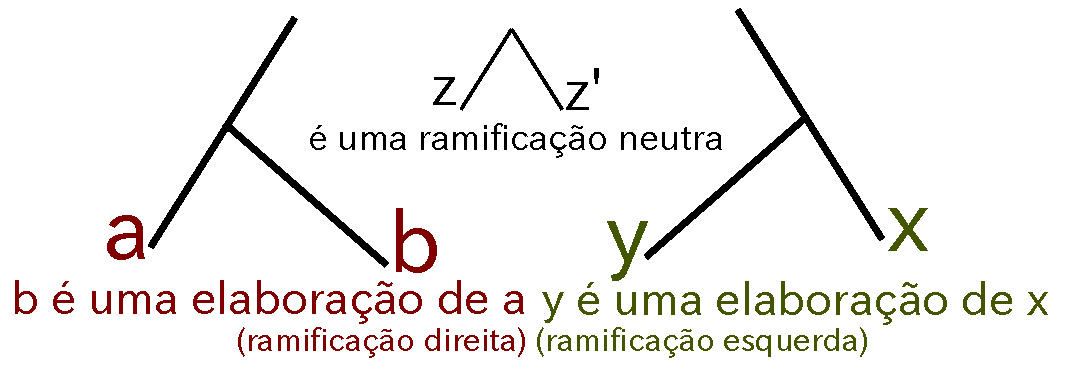
\includegraphics[scale=0.5]{gttm/ramificacoes_arvore.pdf}
	\end{center}
	\legend{Fonte: autor }
\end{figure}







Lerdahl(1996) propõe um modelo de cálculo para medir a intensidade do relaxamento-tensão entre os agrupamentos prolongacionais em todos seus níveis, buscando um modelo quantitativo para inferir os graus.


figura prolongamentos


O modelo mediria a distância entre.... (demonstrar o exemplo do calculating)

O artigo aplica a fórmula para medida de tensão e relaxamento em alguns compassos da sonata K.282 de Mozart(lerdahl 1996 pg.tal). Questionamos se tal ideia de tensão e relaxamento é aplicável nas músicas pós-tonais, onde a condução de vozes pode não estar tão condicionada a esta ideia de prolongamento em função de uma tensão-resolução mas sim a um conceito de agrupamento de sonoridades por outros critérios. 


\section{Cognição das Estruturas Musicais Básicas (CBMS)}



\begin{citacao}
Before beginning to discuss the grammar of grouping structure, we must enter an important caveat. At the present stage of development of the theory, we are treating all music as essentially homophonic; that is, we assume that a single grouping analysis suffices for all voices of a piece. For the more contrapuntal varieties of tonal music, where this condition does not obtain, our theory is inadequate. We consider an extension of the theory to account for polyphonic music to be of great importance. However, we will not attempt to treat such music here except by approximation.\cite{lerdahl1983generative}
\end{citacao}



\subsubsection{Solfejo das Classes de Alturas Tonais}

Temperley justifica esta abordagem por estar buscando um agrupamento das classes de altura que considere os cromatismos fora de uma escala como notas de passagem ou ornamentais dentro de uma função tonal.

A inferência de tonalidade proposta por Lerdahl é inspirada no modelo cognitivista de "distâncias percebidas entre as alturas"(lerdahl 1996 pg.359 paragrafo 3) proposto por Krumsahl(1982,1990), que entre outras propostas constrói histogramas de referência de um "perfil tonal"(krum 1982) dada pelas notas presentes em um segmento.

imagem temperley pg.154



Vejamos por exemplo o perfil do histograma para algumas segmentações de classes de alturas de Mikrokosmos 113[nota m21]:




Segundo tal proposta e as re-elaborações sugeridas por Temperley(2001) pg.173-181, poderíamos tentar inferir uma tonalidade "cognitiva" que permeie os segmentos da peça, buscando agrupar algumas famílias de "eixos paradigmáticos"(nattiez, tripartite, pg.26) a partir de certa tendência que mesmo em dado cromatismo teríamos de associar o segmento a certa tonalidade.

No entanto antes de pensar estas inferências tonais em peças pós-tonais gostaríamos de problematizar abordagens que não estão tão condicionadas por uma suposta cognição tonal predominante. Discutiremos o problema logo a seguir.\footnote{\url{http://web.mit.edu/music21/doc/moduleReference/moduleAnalysisDiscrete.html}} 


\cite{temperley1999s}


\subsubsection{Algoritmo dos Perfis de Tonalidade}
 
Krumhansl Schmuckler 


\scalebox{2}{%
$
r= 
\frac{\sum{(x-\overline{x})(y-\overline{y})}}
{\sqrt{ \sum{ (x-\overline{x})^2 } \sum{ (y-\overline{y})^2 } } }
$
}

For a number of years, it was recognized that the Krumhansl–Kessler key profiles are
similar—but not identical—to the frequency of occurrence for scale degrees in the
actual music. In her landmark 1990 book, Krumhansl argued that this similarity impli-
cates learning-from-exposure. The psychological schemas for the major and minor key
profiles are cognitive reflections of an objective statistical regularity in Western musical
practice. Unfortunately, the evidence seemed imperfect. As we have seen, the domi-
nant is the most frequently occurring pitch in both the major and minor modes, yet
the Krumhansl and Kessler profiles consistently rate the tonic higher than the domi-
nant. In addition, the second and fourth scale degrees (supertonic and subdominant)
are rated significantly less highly than the actual presence of these tones would
suggest. Why do the Krumhansl–Kessler “key profile” distributions differ from the
pitch-class distributions of the music itself?






\section{Restrições Cognitivas versus Segmentação Atonal}


Quase 10 anos após a publicação da GTTM Lerdahl publica um ensaio chamado \textbf{"Restrições cognitivas nos sistemas composicionais"}\cite{lerdahl1992cognitive}\footnote{
Aesthetic Claim 1: The best music utilizes the full potential of our
cognitive resources. Aesthetic Claim 2: The best music arises from an alliance of a compos-
itional grammar with the listening grammar. \cite{lerdahl1992cognitive}
}, ancorando observações em uma aproximação bastante conservadora e crítica da música serial, tomando como caso a peça "Le Marteau Sans Maitre" de Pierre Boulez, e defendendo a tese de que uma música tão distante dos perfis cognitivos básicos da musica tonal seria inapreensível para os sentidos\footnote{Conferir também o ensaio de Milton \citeonline{babbitt1958cares} chamado "Who Cares If you Listen" que argumenta os pressupostos que sustentariam uma pesquisa \textbf{despreocupada da escuta leiga} e que necessita o suporte da ciência para abrir novas fronteiras no desconhecido, assim como ocorre com as ciências exatas não-aplicadas. }. 

Importante levar em conta portanto que a GTTM e suas derivações insistem sempre numa afirmação de uma suposta preferência cognitiva regida pelos princípios "atrativos" tonais, o que pode ser interessante em teorias pós-tonais para pensar ambiguidade de sistemas que induzem uma intenção auditiva politonal, mas não parece ser suficiente para pensar critérios que considerem uma busca auditiva pelas sonoridades de grupos de intervalos não organizados a partir da suposta ordem dos "espaços de alturas tonais"(lerdal 1988,2001) intuídos pela cognição de uma escuta ocidentalizada ou ocidentalizante.

Cabe pensar aqui aquilo que nattiez diferencia como estésica externa e estésica indutiva(nattiez pg.18-20). \textbf{Estésica externa} é aquela baseada em critérios que entrariam na análise por via de uma comprovação de pesquisa de campo, buscando legitimar que os paradigmas apontados são estatisticamente comuns para a percepção de um determinado grupo de ouvintes. Já a \textbf{estésica indutiva} seria determinada por uma inferência explícita e autoral do musicólogo, que aponta aquilo que segundo seus próprios critérios poderia ser percebido como relevante e importante numa escuta. Poderia-se inclusive argumentar um interesse declaradamente apenas estrutural, por aquilo que Nattiez chama de "nível neutro", "análise imanente" ou "análise material" - onde estruturas presentes são destacadas mesmo que possa-se argumentar que foram ali colocadas de maneira inconsciente pelo compositor ou que são imperceptíveis para o ouvinte médio.

Trabalharemos no capítulo seguinte uma abordagem sobre as alturas cromáticas que parte de outros princípios de agrupamento, buscando fórmulas composicionais algorítmicas por meio de uma abordagem que rompe com a normatização  da cultura tonal clássica e busca novos critérios para observar transformações nas alturas e seus agrupamentos.

\begin{citacao}
Where does a compositional grammar come from? The answer varies, but a few
generalizations may be helpful. Let us distinguish between a "natural" and an
"artificial" compositional grammar. A natural grammar arises spontaneously in
a musical culture. An artificial grammar is the conscious invention of an indi-
vidual or group within a culture. The two mix fruitfully in a complex and long-
lived musical culture such as that of Western tonality. A natural grammar will
dominate in a culture emphasizing improvisation and encouraging active partici-
pation of the community in all the varieties of musical behaviour. An artificial
grammar will tend to dominate in a culture that utilizes musical notation, that is
self-conscious, and that separates musical activity into composer, performer,
and listener.
\cite[p. 100-101]{lerdahl1992cognitive}
\end{citacao}








Temperley adopts the plan outlined by Krumhansl and Schmuckler (de- 
scribed in Krumhansl, 1990): (1) segment a composition into small sections, (2) tally 
the tones within a segment (weighting each pitch class by its total duration as well 
as by other possible measures of salience), (3) mathematically correlate the vector 
of tone tallies with the tone-profile vectors for all twenty-four major and minor keys, 
and (4) select the highest correlation as the best candidate for representing the per- 
ceived key of that segment. 



Lerdahl logo em seguida flerta com musica atonal, etc... \cite{lerdahl1992cognitive} antes de buscar sua atualização da teoria após a influencia das teorias de Forte, Babbit e outros na musicologia americana influencia da teoria de grupos (o que foge um pouco de nosso escopo)  e sim no próximo capitulo buscar um entendimento básico da eoria de grupos blabla


abaixo um esquema feito por ele no seu artigo de revisão da GTTM
%%%%%%%%%%%%%%%%%% tonal pitch space
\begin{figure}[!h]
	\caption{\label{fig_grafico}Extensão das regras de GTTM na obra “Tonal Pitch Space” propostas por \citeonline{lerdahl2009genesis} }
	\begin{center}
	    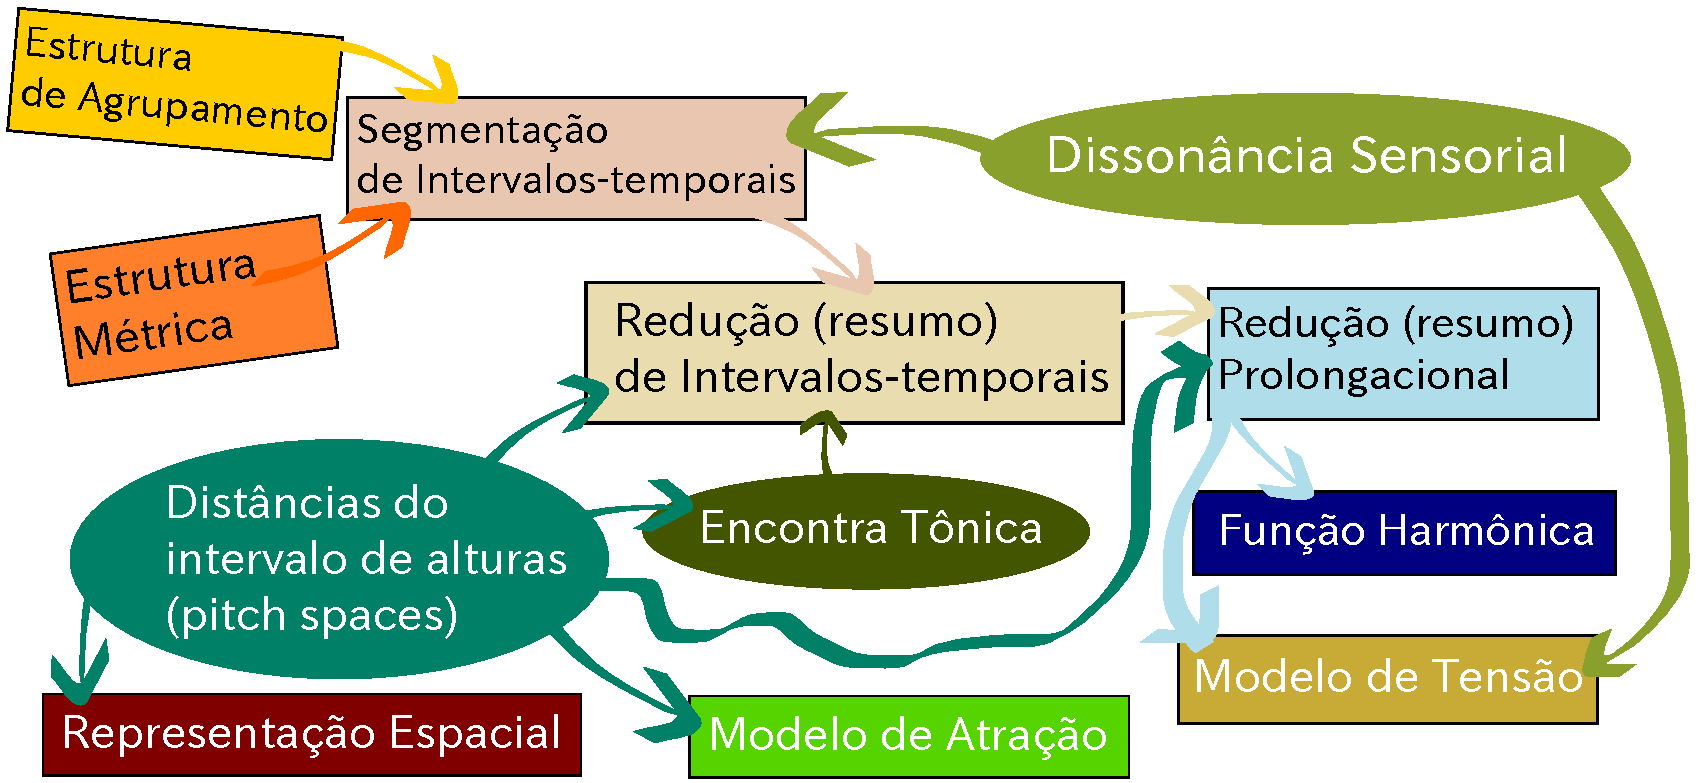
\includegraphics[scale=0.5]{gttm/GTTM_TPS_rules.pdf}
	\end{center}
	\legend{Fonte: \cite[ tradução do autor.]{lerdahl2009genesis} }
\end{figure}


\begin{citacao}
The ideological desperation of the Lerdahl–Jackendoff commitment to tonality as somehow embedded in human nature is exposed in the simple activity of natural speech. People in normal conversation speak in atonal cadences because to do otherwise would be personally tiresome as well as expose them to ridicule.
Angular melodies of Schoenberg, Webern, or Mozart are more naturalistic than conventionalsong. Formal speech is explicitly atonal.
\end{citacao}







\chapter{Teorias de Grupos das Classes de Alturas para uma Segmentação Atonal }
\label{modelos}

Vimos na teoria do "solfejo das classes de altura"\cite[p. 115]{temperley2004cognition} de David \citeonline{temperley2004cognition} a categorização de uma divisão de grupos de altura que ele denomina "Altura de Classes Tonais"\cite[p. 115]{temperley2004cognition}. Neste capítulo exploramos teorias pós-tonais que são geralmente evitadas pela abordagem cognitivista por partirem de princípios de agrupamento que não são argumentados por uma funcionalidade tonal normativa, mas sim pela formalização de relações de simetria, similaridade e transformação entre os doze intervalos cromáticos que trariam o sentido musical por outros tipos de fruição da forma musical. 

Na teoria de grupos de classes de altura ("Pitch Class Theory") os intervalos são tratados de maneira neutra em relação a qualquer centro tonal pré-determinado e parte-se do princípio de que agrupamentos de alturas podem gerar estruturas de derivadas por uma espécie de parentesco intervalar, incluindo a similaridade por inversão ou retrógrado destes como veremos mais adiante. 

Estas teorias são fortemente influenciadas pela ideia de serialismo formalizada pelo dodecafonismo frequentemente atribuído a Arnold Shoenberg e seus pupilos da segunda escola de Vienna, mas é bom lembrar que o pensamento serial é um pensamento composicional que pode também ser encontrado em compositores muito anteriores a estas formalizações, portanto podemos encontrar esta abordagem analítica sendo usada para destacar aspectos de composições de outros contextos que não o restrito ao repertório atonal clássico, como faz por exemplo Joel \citeonline{lester1989analytic} em sua didática para análises de um repertório pós-tonal do ínicio do século XX ou Allen Forte na sua tese sobre a "Sagração da Primavera" de Stravinski\cite{forte1978harmonic}.

\begin{citacao}
It was, of course, Allen Forte who in the USA pioneered the analytical with a taxonomy of pc-set application of concepts from mathematics, first arose also in serial Babbittian types (the concept theory), and following as
some inclusion and with relations abstract up (such similarity relations) meant for analytical use. Forte's "set theory" (as it is somewhat misleadingly known, because it deals with sets of pitch classes) has had its own
ramifications and influence. In particular, Forte's own analyses of individual pieces of music have led many others to do likewise, and Forte's initial idea of similarity relations (as distinct from equivalence relations) among pitch-class sets has seen a flourishing theoretical industry grow around it, after seminal articles by Morris, Rahn, and Lewin appeared in 1980.\cite{rahn2004swerve}
\end{citacao}



Com formalização de uma teoria de grupos de classes de alturas pela geração de musicólogos e compositores seriais da segunda metade do século XX e com os avanços exponenciais da computação nas últimas décadas estas teorias vão sendo testadas e aplicadas computacionalmente a ponto de já constituírem uma área bastante específica da musicologia contemporânea. 

Um exemplo de interesse do presente trabalho é a classe de objetos "Math Tools"\cite{andreatta2003implementing,AndreataOMtutorial,DebrilOM} da linguagem de programação OpenMusic, que organiza em orientação a objetos muitos dos conceitos que veremos logo a seguir. 








\section{Formulas de canonizaç~ao e transformaç~ao dos intervalos}



\citeonline{straus2004}







\subsection{Forma Prima}

\begin{citacao}
Two Algorithms for Computing the Prime Form

There are two algorithms for computing the prime form of a Pitch Class Set. The first was introduced by Allen Forte in The Structure of Atonal Music and the second is used by John Rahn in his book Basic Atonal Theory and is also used by Joseph N. Straus in his Introduction to Post-Tonal Theory.

The difference between the two algorithms is apparent when examining Pitch Class Set 6-31. The Prime Form using the Forte algorithm is (0,1,3,5,8,9), and the prime form using the Rahn algorithm is (0,1,4,5,7,9). As you can see, the Forte algorithm puts a priority on making the small numbers smaller (i.e. 3 instead of 4), whereas the Rahn algorithm wants the larger numbers to be smaller (i.e. 7 instead of 8).

Which is better? Well, it depends on who you ask. Computer programmers and computer music people will typically prefer the Rahn algorithm because it is computationally more elegant. However, the Forte algorithm has the more established pedigree, and so it tends to be preferred by academics.

Fortunately, this is usually a minor issue because it only affects the following 5 sets:

Pitch Class Set	Forte Prime	Rahn Prime
5-20	(0,1,3,7,8)	(0,1,5,6,8)
6-Z29	(0,1,3,6,8,9)	(0,2,3,6,7,9)
6-31	(0,1,3,5,8,9)	(0,1,4,5,7,9)
7-20	(0,1,2,4,7,8,9)	(0,1,2,5,6,7,9)
8-26	(0,1,2,4,5,7,9,10)	(0,1,3,4,5,7,8,10)
\end{citacao}


% ---
\chapter{Analises aplicadas}
% ---
\label{experimetosanalises}

mikro 131 133 simetria
\cite[pgs.198-200]{antokoletz1984music}

mikro 101 109 150 polimodalismo octatonismo 
\cite[pgs.250-254]{antokoletz1984music}



"Diminished Fifth" a obra nº101 da suíte Mikrokosmos de Béla Bartók.\cite[pgs.112,116-117,135-136]{lester1989analytic}.








\section{Analise de Mikrokosmos 113 Bela Bartok}

%\begin{comment}
%%%%%%%%%%%%%%%intro mikro
\begin{figure}[htb]
	\caption{\label{fig_grafico}Legatto das melodias sugere a segmentação}
	\begin{center}
	    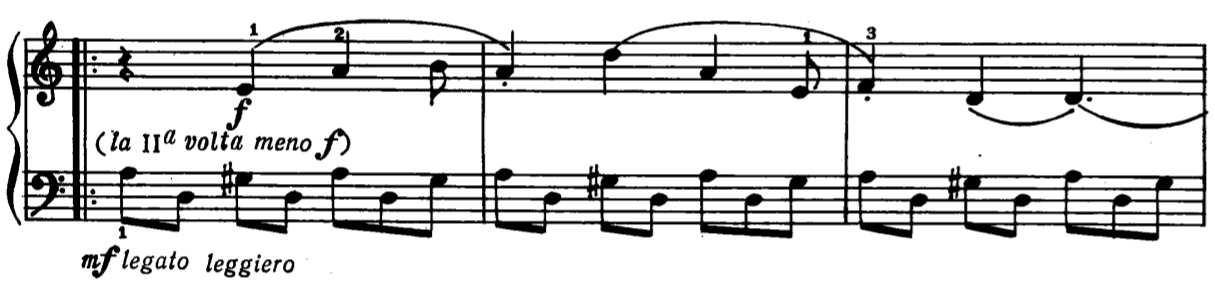
\includegraphics[scale=0.35]{mikro/mikro113-intro.png}
	\end{center}
	%\legend{Fonte: autor}
\end{figure}
%%%%%%%%%%%%%%%%%%%%%%%%%%%%%%

%%%%%%%%%%%%%%%segmentação mikro
\begin{figure}[htb]
	\caption{\label{fig_grafico}Segmentação em árvore prolongacional de Mikrokosmos 113 ao estilo GTTM}
	\begin{center}
	    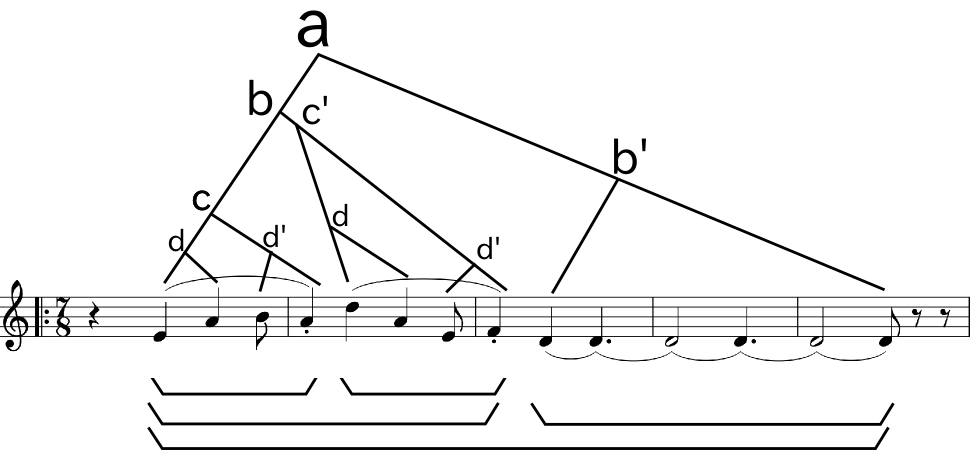
\includegraphics[scale=0.45]{mikro/mikro113_GTTM_tree.png}
	\end{center}
	\legend{Fonte: autor}
\end{figure}
%%%%%%%%%%%%%%%%%%%%%%%%%%%%%%






%%%%%%%%%%%%%%pitch por secção%%%%%%%%%%%%%%%%%%%%%%%%%%
\begin{figure}[htb]
% \label{ }
 \centering
  \begin{minipage}{0.4\textwidth}
    \centering
    \caption{Secção A} \label{fig_minipage_imagem1}
    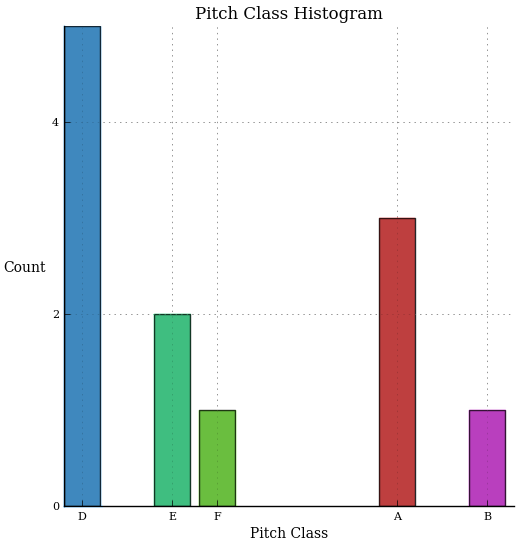
\includegraphics[scale=0.6]{mikro/A.png}
    %\legend{ }
  \end{minipage}
  \hfill
  \begin{minipage}{0.4\textwidth}
    \centering
    \caption{Secção B} \label{fig_minipage_grafico2}
    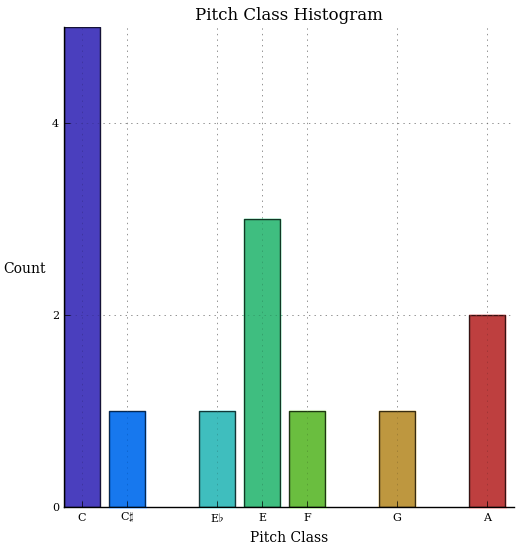
\includegraphics[scale=0.6]{mikro/B.png}
    %\legend{ }
  \end{minipage}
\end{figure}
%%%%%%%%%%%%%%%%%%%
\begin{figure}[htb]
% \label{ }
 \centering
  \begin{minipage}{0.4\textwidth}
    \centering
    \caption{Secção C} \label{fig_minipage_imagem1}
    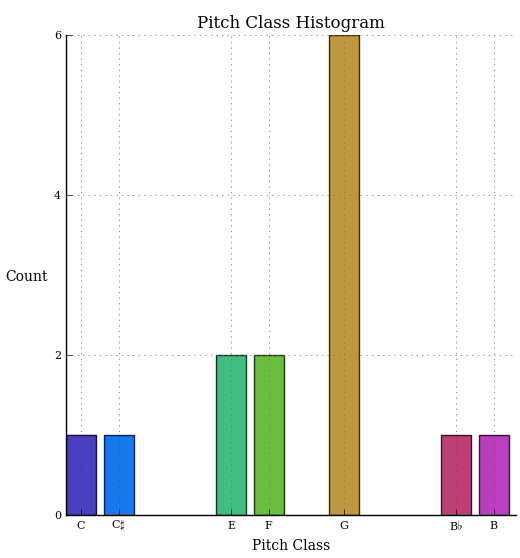
\includegraphics[scale=0.6]{mikro/C.png}
    %\legend{ }
  \end{minipage}
  \hfill
  \begin{minipage}{0.4\textwidth}
    \centering
    \caption{Secção D} \label{fig_minipage_grafico2}
    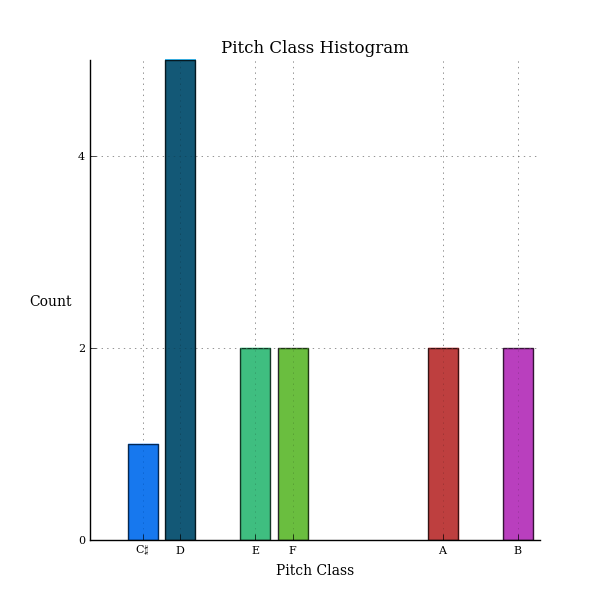
\includegraphics[scale=0.6]{mikro/D.png}
    %\legend{ }
  \end{minipage}
\end{figure}
\pagebreak
%%%%%%%%%%%%%%%%%%%%%%%%%%%%%%%%%%%%%%%%%%%%%%%%%

%%%% analise das seções por condução de vozes
\begin{figure}[htb]
	\caption{\label{fig_grafico}Análise das seções por condução de vozes}
	\begin{center}
	    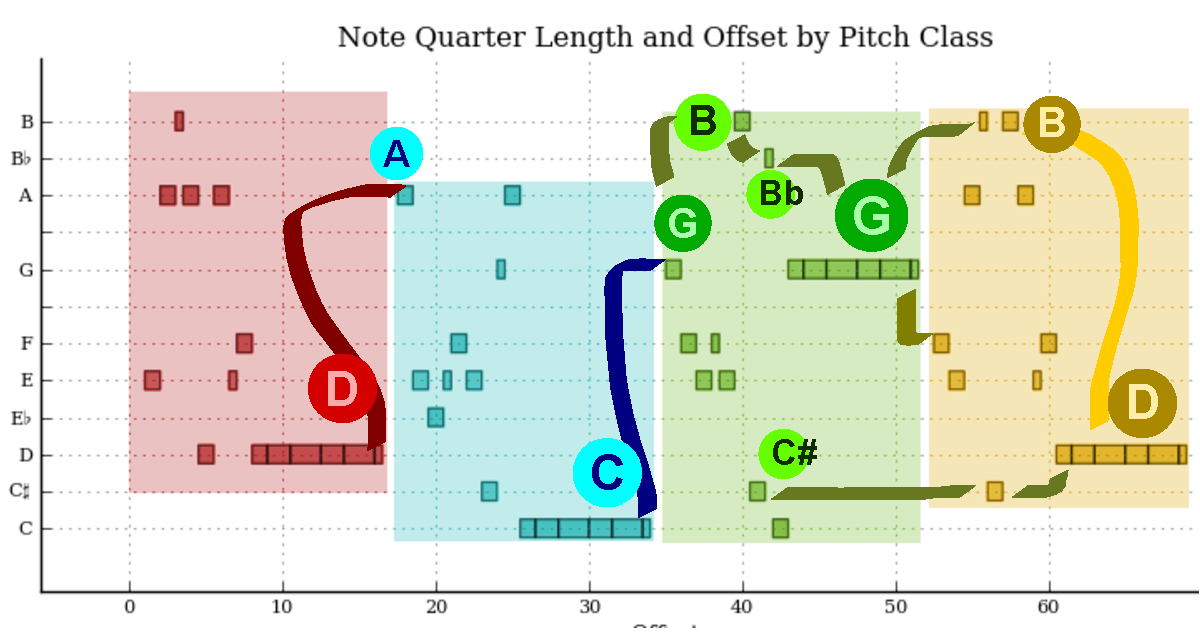
\includegraphics[scale=0.75]{mikro/mikrokosmos113-prolongational.pdf}
	\end{center}
	\legend{Fonte: autor}
\end{figure}
%%%%%%%%%%%%%%%%%%%%%%%%%%%%%%%%%%%%%%%%%%%%%%%%%%%%%%%%%%%%%%%%%%


%%%%%%%%%%pitch space melodia
\begin{figure}[htb]
	\caption{\label{fig_grafico}Pitch space melodia}
	\begin{center}
	    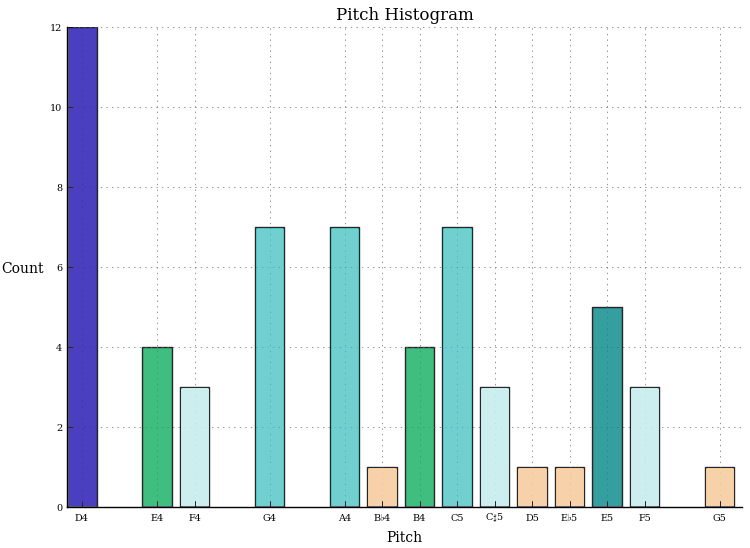
\includegraphics[scale=0.45]{mikro/mikro_melodia_pitch_space.png}
	\end{center}
	\legend{Fonte: autor}
\end{figure}
%%%%%%%%%%%%%%%%%%%%%%%%%%%%%%%%%%%
%\end{comment}





\part{Luteria Composicional}
\label{composicional}

\chapter{Aplicação de estruturas sugeridas pelas análises musicais em procedimentos algorítmicos clássicos}




% ----------------------------------------------------------
% Finaliza a parte no bookmark do PDF
% para que se inicie o bookmark na raiz
% e adiciona espaço de parte no Sumário
% ----------------------------------------------------------
\phantompart

% ---
% Conclusão (outro exemplo de capítulo sem numeração e presente no sumário)
% ---
\chapter*[Conclusão]{Conclusão}
\addcontentsline{toc}{chapter}{Conclusão}
% ---

\lipsum[31-33]

% ----------------------------------------------------------
% ELEMENTOS PÓS-TEXTUAIS
% ----------------------------------------------------------
\postextual
% ----------------------------------------------------------

% ----------------------------------------------------------
% Referências bibliográficas
% ----------------------------------------------------------
%\bibliography{abntex2-modelo-references}
\bibliography{mestrado_glerm}
% ----------------------------------------------------------
% Glossário
% ----------------------------------------------------------
%
% Consulte o manual da classe abntex2 para orientações sobre o glossário.
%
%\glossary

% ----------------------------------------------------------
% Apêndices
% ----------------------------------------------------------

% ---
% Inicia os apêndices
% ---
\begin{apendicesenv}

% Imprime uma página indicando o início dos apêndices
\partapendices




%%%%

\chapter{Repositório de Códigos}
\label{codigo}


\subsection{Biblioteca de Algoritmos}



\lstset{frameround=fttt,language=Python,showspaces=false,
showtabs=true,tab=\rightarrowfill}
\begin{lstlisting}[frame=trBL]
def mod12(n):
	return n % 12

def note_name(number):
	notes = "C  D E F G A B".split()
	return notes[mod12(number)]
	
for i in intervalos:
	if (i in maiores):
		if (i == (4,7)):
			tipos.append(("maior",0))
		if (i == (5,9)):
			tipos.append(("maior",1))
		if (i == (3,8)):
			tipos.append(("maior",2))
 
	if (i in menores):
		if (i == (3,7)):
			tipos.append(("menor",0))
		if (i == (5,8)):
			tipos.append(("menor",1))
		if (i == (4,9)):
			tipos.append(("menor",2))
	if (i in aumentados):
			tipos.append(("aumentado","not"))
	if (i in diminutos):
		if (i == (3,6)):
			tipos.append(("diminuto",0))
		if (i == (6,9)):
			tipos.append(("diminuto",1))
		if (i == (3,9)):
			tipos.append(("diminuto",2))
 
\end{lstlisting}





\end{apendicesenv}
% ---


% ----------------------------------------------------------
% Anexos
% ----------------------------------------------------------

% ---
% Inicia os anexos
% ---
\begin{anexosenv}

% Imprime uma página indicando o início dos anexos
\partanexos

\chapter{Tabela de Pitch Class Set de Allen Forte}
\label{forte}

\begin{table}[h]
\begin{tabular}{lllll}
\# & Fortecross-referenced Set-name & Prime & Interval Vector & Descriptive name/properties                       \\
0  & 0-1                            & empty & 000000          & Null set                                          \\
1  & 1-1*                           & 0     & 000000          & Unison                                            \\
2  & 2-1*                           & 01    & 100000          & Semitone                                          \\
3  & 2-2*                           & 02    & 010000          & Whole-tone                                        \\
4  & 2-3*                           & 03    & 001000          & Minor Third                                       \\
5  & 2-4*                           & 04    & 000100          & Major Third                                       \\
6  & 2-5*                           & 05    & 000010          & Perfect Fourth                                    \\
7  & 2-6*(6)                        & 06    & 000001          & Tritone                                           \\
8  & 3-1*                           & 012   & 210000          & BACH /Chromatic Trimirror                         \\
9  & 3-2                            & 013   & 111000          & Phrygian Trichord                                 \\
10 & 3-2B                           & 023   & 111000          & Minor Trichord                                    \\
11 & 3-3                            & 014   & 101100          & Major-minor Trichord.1                            \\
12 & 3-3B                           & 034   & 101100          & Major-minor Trichord.2                            \\
13 & 3-4                            & 015   & 100110          & Incomplete Major-seventh Chord.1                  \\
14 & 3-4B                           & 045   & 100110          & Incomplete Major-seventh Chord.2                  \\
15 & 3-5                            & 016   & 100011          & Rite chord.2, Tritone-fourth.1                    \\
16 & 3-5B                           & 056   & 100011          & Rite chord.1, Tritone-fourth.2                    \\
17 & 3-6*                           & 024   & 020100          & Whole-tone Trichord                               \\
18 & 3-7                            & 025   & 011010          & Incomplete Minor-seventh Chord                    \\
19 & 3-7B                           & 035   & 011010          & Incomplete Dominant-seventh Chord.2               \\
20 & 3-8                            & 026   & 010101          & Incomplete Dominant-seventh Chord.1/Italian-sixth \\
21 & 3-8B                           & 046   & 010101          & Incomplete Half-dim-seventh Chord                 \\
22 & 3-9*                           & 027   & 010020          & Quartal Trichord                                  \\
23 & 3-10*                          & 036   & 002001          & Diminished Chord                                  \\
24 & 3-11                           & 037   & 001110          & Minor Chord                                       \\
25 & 3-11B                          & 047   & 001110          & Major Chord                                       \\
26 & 3-12*(4)                       & 048   & 000300          & Augmented Chord                                   \\
27 & 4-1*                           & 0123  & 321000          & BACH /Chromatic Tetramirror                       \\
28 & 4-2                            & 0124  & 221100          & Major-second Tetracluster.2                       \\
29 & 4-2B                           & 0234  & 221100          & Major-second Tetracluster.1                       \\
30 & 4-3*                           & 0134  & 212100          & Alternating Tetramirror                           \\
31 & 4-4                            & 0125  & 211110          & Minor Third Tetracluster.2                        \\
32 & 4-4B                           & 0345  & 211110          & Minor Third Tetracluster.1                        \\
33 & 4-5                            & 0126  & 210111          & Major Third Tetracluster.2                        \\
34 & 4-5B                           & 0456  & 210111          & Major Third Tetracluster.1                        \\
35 & 4-6*                           & 0127  & 210021          & Perfect Fourth Tetramirror                        \\
36 & 4-7*                           & 0145  & 201210          & Arabian Tetramirror                               \\
37 & 4-8*                           & 0156  & 200121          & Double Fourth Tetramirror                         \\
38 & 4-9*(6)                        & 0167  & 200022          & Double Tritone Tetramirror                        \\
39 & 4-10*                          & 0235  & 122010          & Minor Tetramirror                                 \\
40 & 4-11                           & 0135  & 121110          & Phrygian Tetrachord                               \\
41 & 4-11B                          & 0245  & 121110          & Major Tetrachord                                  \\
42 & 4-12\textless                  & 0236  & 112101          & Harmonic-minor Tetrachord                         \\
43 & 4-12B\textless                 & 0346  & 112101          & Major-third Diminished Tetrachord                 \\
44 & 4-13                           & 0136  & 112011          & Minor-second Diminished Tetrachord                \\
45 & 4-13B                          & 0356  & 112011          & Perfect-fourth Diminished Tetrachord              \\
46 & 4-14\textless                  & 0237  & 111120          & Major-second Minor Tetrachord                     \\
47 & 4-14B\textless                 & 0457  & 111120          & Perfect-fourth Major Tetrachord                   \\
48 & 4-Z15..29                      & 0146  & 111111          & All-interval Tetrachord.1                         \\
49 & 4-Z15B..29                     & 0256  & 111111          & All-interval Tetrachord.2                         \\
\end{tabular}
\end{table}



\pagebreak
\begin{table}[h]
\begin{tabular}{lllll}
50 & 4-16                           & 0157  & 110121          & Minor-second Quartal Tetrachord                   \\
51 & 4-16B                          & 0267  & 110121          & Tritone Quartal Tetrachord                        \\
52 & 4-17*                          & 0347  & 102210          & Major-minor Tetramirror                           \\
53 & 4-18                           & 0147  & 102111          & Major-diminished Tetrachord                       \\
54 & 4-18B                          & 0367  & 102111          & Minor-diminished Tetrachord                       \\
55 & 4-19                           & 0148  & 101310          & Minor-augmented Tetrachord                        \\
56 & 4-19B                          & 0348  & 101310          & Augmented-major Tetrachord                        \\
57 & 4-20*                          & 0158  & 101220          & Major-seventh Chord                               \\
58 & 4-21*                          & 0246  & 030201          & Whole-tone Tetramirror                            \\
59 & 4-22                           & 0247  & 021120          & Major-second Major Tetrachord                     \\
60 & 4-22B                          & 0357  & 021120          & Perfect-fourth Minor Tetrachord                   \\
61 & 4-23*                          & 0257  & 021030          & Quartal Tetramirror                               \\
62 & 4-24*                          & 0248  & 020301          & Augmented Seventh Chord                           \\
63 & 4-25*(6)                       & 0268  & 020202          & French-sixth Chord                                \\
64 & 4-26*                          & 0358  & 012120          & Minor-seventh Chord                               \\
65 & 4-27                           & 0258  & 012111          & Half-diminished Seventh Chord                     \\
66 & 4-27B                          & 0368  & 012111          & Dominant-seventh/German-sixth Chord               \\
67 & 4-28*(3)                       & 0369  & 004002          & Diminished-seventh Chord                          \\
68 & 4-Z29..15                      & 0137  & 111111          & All-interval Tetrachord.3                         \\
69 & 4-Z29B..15                     & 0467  & 111111          & All-interval Tetrachord.4                         \\
70 & 5-1*                           & 01234 & 432100          & Chromatic Pentamirror                             \\
71 & 5-2                            & 01235 & 332110          & Major-second Pentacluster.2                       \\
72 & 5-2B                           & 02345 & 332110          & Major-second Pentacluster.1                       \\
73 & 5-3                            & 01245 & 322210          & Minor-second Major Pentachord                     \\
74 & 5-3B                           & 01345 & 322210          & Spanish Pentacluster                              \\
75 & 5-4                            & 01236 & 322111          & Blues Pentacluster                                \\
76 & 5-4B                           & 03456 & 322111          & Minor-third Pentacluster                          \\
77 & 5-5                            & 01237 & 321121          & Major-third Pentacluster.2                        \\
78 & 5-5B                           & 04567 & 321121          & Major-third Pentacluster.1                        \\
79 & 5-6                            & 01256 & 311221          & Oriental Pentacluster.1, Raga Megharanji (13161)  \\
80 & 5-6B                           & 01456 & 311221          & Oriental Pentacluster.2                           \\
81 & 5-7                            & 01267 & 310132          & DoublePentacluster.1, Raga Nabhomani (11415)      \\
82 & 5-7B                           & 01567 & 310132          & Double Pentacluster.2                             \\
83 & 5-8*                           & 02346 & 232201          & Tritone-Symmetric Pentamirror                     \\
84 & 5-9                            & 01246 & 231211          & Tritone-Expanding Pentachord                      \\
85 & 5-9B                           & 02456 & 231211          & Tritone-Contracting Pentachord                    \\
86 & 5-10                           & 01346 & 223111          & Alternating Pentachord.1                          \\
87 & 5-10B                          & 02356 & 223111          & Alternating Pentachord.2                          \\
88 & 5-11                           & 02347 & 222220          & Center-cluster Pentachord.1                       \\
89 & 5-11B                          & 03457 & 222220          & Center-cluster Pentachord.2                       \\
90 & 5-Z12*..36                     & 01356 & 222121          & Locrian Pentamirror                               \\
91 & 5-13                           & 01248 & 221311          & Augmented Pentacluster.1                          \\
92 & 5-13B                          & 02348 & 221311          & Augmented Pentacluster.2                          \\
93 & 5-14                           & 01257 & 221131          & Double-seconds Triple-fourth Pentachord.1         \\
94 & 5-14B                          & 02567 & 221131          & Double-seconds Triple-fourth Pentachord.2         \\
95 & 5-15*                          & 01268 & 220222          & Assymetric Pentamirror                            \\
96 & 5-16                           & 01347 & 213211          & Major-minor-dim Pentachord.1                      \\
97 & 5-16B                          & 03467 & 213211          & Major-minor-dim Pentachord.2                      \\
98 & 5-Z17*..37                     & 01348 & 212320          & Minor-major Ninth Chord                           \\
99 & 5-Z18\textless..38             & 01457 & 212221          & Gypsy Pentachord.1                               

\end{tabular}
\end{table}


% ---
\chapter{Regras da Teoria Gerativa da Musica Tonal}
% ---


\end{anexosenv}

%---------------------------------------------------------------------
% INDICE REMISSIVO
%---------------------------------------------------------------------
\phantompart
\printindex
%---------------------------------------------------------------------

\end{document}
